% !TeX root = ../do-an.tex
% CHUONG 3 - PHAN TICH VA THIET KE HE THONG
% Su dung cac hinh PNG trong thu muc assets/

\chapter{Phân tích và thiết kế hệ thống}
\setlength{\parindent}{0pt}

% =========================================================
% 3.1 PHÂN TÍCH BÀI TOÁN
% =========================================================

\Needspace{12\baselineskip}
\section{Phân tích bài toán}

\Needspace{9\baselineskip}
\subsection{Đặt vấn đề}

Thực phẩm là một phần thiết yếu trong đời sống hằng ngày. Tuy nhiên, đối với những người có cơ địa dị ứng thực phẩm, việc lựa chọn sản phẩm cần được thực hiện cẩn thận. Một số thành phần như sữa, trứng, đậu nành, đậu phộng, cá, giáp xác, các loại hạt và lúa mì có thể gây phản ứng dị ứng ở những người nhạy cảm.

Trên bao bì thực phẩm, thông tin thành phần thường được trình bày dưới dạng văn bản với kích thước chữ nhỏ. Một số sản phẩm nhập khẩu sử dụng tiếng Anh, tiếng Pháp, tiếng Đức hoặc ngôn ngữ khác. Điều này gây khó khăn cho người dùng khi đọc và xác định thành phần cần tránh. Bên cạnh đó, hình ảnh nhãn thực phẩm có thể bị mờ, thiếu sáng, nghiêng hoặc chứa nhiều thông tin không liên quan.

Từ thực tế đó, đề tài ``Xây dựng hệ thống đọc nhãn mác và cảnh báo thành phần dị ứng thực phẩm'' được thực hiện nhằm hỗ trợ người dùng trích xuất thông tin từ ảnh nhãn thực phẩm, phân tích thành phần và cảnh báo các dị nguyên có liên quan.

Hệ thống Allergy Warning được xây dựng dưới dạng ứng dụng web. Người dùng có thể đăng ký, đăng nhập, lựa chọn các dị nguyên quan tâm trong hồ sơ cá nhân, tải ảnh nhãn thực phẩm lên để phân tích và xem lại lịch sử quét. Hệ thống sử dụng dữ liệu sản phẩm, danh sách dị nguyên và kết quả phân tích để hỗ trợ người dùng nhận biết những thành phần cần chú ý.

\Needspace{9\baselineskip}
\subsection{Mục tiêu phân tích}

Mục tiêu của quá trình phân tích và thiết kế là xác định các chức năng, dữ liệu và thành phần cần thiết để xây dựng hệ thống.

\textbf{Mục tiêu thứ nhất: Tiếp nhận và đọc ảnh nhãn thực phẩm.}

Hệ thống cho phép người dùng tải ảnh nhãn thực phẩm từ thiết bị. Ảnh được đưa vào quy trình xử lý nhằm trích xuất các thông tin có liên quan đến tên sản phẩm, thương hiệu và danh sách thành phần.

\textbf{Mục tiêu thứ hai: Phân tích thông tin thành phần.}

Thông tin trên ảnh nhãn được Gemini API hỗ trợ nhận diện và trích xuất. Nội dung nhận diện, đặc biệt là tên sản phẩm, thương hiệu, danh sách thành phần và thông tin cảnh báo trên nhãn, được chuẩn hóa trước khi đối chiếu với dữ liệu dị nguyên.

\textbf{Mục tiêu thứ ba: Phân biệt các loại cảnh báo.}

Hệ thống cần phân biệt thành phần có bằng chứng xuất hiện trong danh sách thành phần với thông tin cảnh báo có thể chứa vết dị nguyên trên nhãn. Hai trường hợp này có ý nghĩa khác nhau và không nên được trình bày như cùng một kết luận.

\textbf{Mục tiêu thứ tư: Cá nhân hóa kết quả cảnh báo.}

Người dùng có thể lựa chọn các dị nguyên cần chú ý trong hồ sơ cá nhân. Thông tin này được sử dụng để hỗ trợ việc đối chiếu kết quả phân tích với nhu cầu của từng người dùng.

\textbf{Mục tiêu thứ năm: Lưu trữ và tra cứu thông tin.}

Hệ thống lưu thông tin tài khoản, dữ liệu dị nguyên, sản phẩm, thành phần sản phẩm, hồ sơ dị ứng và lịch sử quét trong cơ sở dữ liệu có khả năng tương thích với MySQL. Trong môi trường phát triển, hệ thống có thể sử dụng MySQL/MariaDB; khi triển khai, dữ liệu được lưu trên TiDB Cloud theo cấu hình kết nối của ứng dụng.

\Needspace{9\baselineskip}
\subsection{Phạm vi của hệ thống}

Hệ thống tập trung vào việc đọc nhãn thực phẩm từ ảnh, trích xuất thông tin, đối chiếu dữ liệu dị nguyên và hiển thị cảnh báo. Dữ liệu sản phẩm có thể được lưu trong cơ sở dữ liệu nội bộ hoặc được thu thập từ nguồn dữ liệu sản phẩm như Open Food Facts.

Kết quả phụ thuộc vào chất lượng ảnh, khả năng trích xuất văn bản, dữ liệu có sẵn và quy tắc đối chiếu. Hệ thống chỉ hỗ trợ người dùng tham khảo thông tin trên nhãn, không thay thế việc đọc nhãn gốc, tư vấn y tế hoặc xác nhận an toàn tuyệt đối của sản phẩm.

% =========================================================
% 3.2 KHẢO SÁT VÀ XÁC ĐỊNH YÊU CẦU
% =========================================================

\Needspace{12\baselineskip}
\section{Khảo sát và xác định yêu cầu hệ thống}

\Needspace{9\baselineskip}
\subsection{Đối tượng sử dụng}

\textbf{Người dùng thông thường:}

Người dùng là đối tượng chính của hệ thống. Người dùng có thể tạo tài khoản, đăng nhập, quản lý hồ sơ dị ứng cá nhân, tải ảnh nhãn thực phẩm để phân tích, xem kết quả và tra cứu lịch sử quét của mình.

\textbf{Quản trị viên:}

Quản trị viên là người được cấp quyền truy cập khu vực quản trị. Thông qua giao diện quản trị, quản trị viên có thể theo dõi Dashboard và thực hiện các thao tác quản lý dữ liệu sản phẩm, dữ liệu liên quan theo những chức năng đã được triển khai trong hệ thống.

\Needspace{9\baselineskip}
\subsection{Yêu cầu chức năng}

\textbf{Chức năng đăng ký tài khoản:}

Cho phép người dùng tạo tài khoản bằng thông tin họ tên, email và mật khẩu. Hệ thống kiểm tra dữ liệu đầu vào và lưu thông tin tài khoản vào cơ sở dữ liệu khi đăng ký hợp lệ.

\textbf{Chức năng đăng nhập:}

Cho phép người dùng nhập email và mật khẩu để xác thực. Khi thông tin hợp lệ, người dùng có thể truy cập các chức năng yêu cầu đăng nhập.

\textbf{Chức năng quản lý hồ sơ cá nhân:}

Hiển thị thông tin tài khoản, bao gồm họ tên và email. Người dùng có thể truy cập khu vực hồ sơ để xem và cập nhật thông tin cá nhân theo chức năng được cung cấp.

\textbf{Chức năng quản lý hồ sơ dị ứng:}

Hệ thống cung cấp danh sách các nhóm dị nguyên như sữa, đậu phộng, đậu nành, trứng, cá, giáp xác, động vật thân mềm, hạt cây, lúa mì, mè, mù tạt, cần tây, đậu lupin và sulfit. Người dùng lựa chọn các mục phù hợp với nhu cầu của mình. Những lựa chọn này được lưu trong bảng \texttt{user\_allergens}.

\textbf{Chức năng tải ảnh nhãn thực phẩm:}

Cho phép người dùng chọn ảnh nhãn thực phẩm từ thiết bị và gửi lên hệ thống. Giao diện hiển thị ảnh hoặc tên ảnh đã chọn và cung cấp thao tác bắt đầu phân tích.

\textbf{Chức năng trích xuất thông tin từ ảnh:}

Hệ thống tiếp nhận ảnh và thực hiện quá trình nhận diện thông tin. Nội dung thu được có thể bao gồm tên sản phẩm, thương hiệu, thành phần và thông tin dị nguyên trên nhãn.

\textbf{Chức năng phân tích thành phần:}

Hệ thống phân tích danh sách thành phần thu được, sau đó đối chiếu với dữ liệu dị nguyên. Những nội dung phù hợp với quy tắc đối chiếu được tổng hợp để phục vụ quá trình cảnh báo.

\textbf{Chức năng cảnh báo dị nguyên:}

Kết quả được chia thành các trường hợp có thành phần liên quan đến dị nguyên và trường hợp có cảnh báo có thể chứa vết dị nguyên. Hệ thống hiển thị tên dị nguyên cùng bằng chứng liên quan để người dùng dễ theo dõi.

\textbf{Chức năng hiển thị kết quả:}

Giao diện kết quả hiển thị tên sản phẩm, thương hiệu, ảnh sản phẩm, danh sách thành phần được nhận diện, các dị nguyên và trạng thái cảnh báo.

\textbf{Chức năng lưu lịch sử quét:}

Hệ thống lưu thông tin mỗi lần quét trong bảng \texttt{scan\_history}, bao gồm mã lần quét, người thực hiện, sản phẩm, ảnh, thành phần, dị nguyên, cảnh báo và thời điểm quét.

\textbf{Chức năng xem lịch sử quét:}

Cho phép người dùng xem lại các sản phẩm đã phân tích và trạng thái cảnh báo của những lần quét trước đó. Người dùng có thể mở chi tiết một lần quét để xem thông tin được lưu.

\textbf{Chức năng quản lý dữ liệu dành cho quản trị viên:}

Khu vực quản trị cung cấp giao diện Dashboard và các màn hình dữ liệu. Tùy theo quyền được cấp, quản trị viên có thể theo dõi thông tin tổng quan, xem dữ liệu sản phẩm, xem chi tiết sản phẩm và kiểm tra các dữ liệu được hệ thống quản lý.

\textbf{Chức năng tra cứu dữ liệu sản phẩm:}

Hệ thống lưu thông tin sản phẩm trong bảng \texttt{products}. Dữ liệu này có thể được dùng để đối chiếu với sản phẩm đã biết khi có thông tin phù hợp, chẳng hạn mã vạch hoặc thông tin nhận diện sản phẩm.

\Needspace{9\baselineskip}
\subsection{Yêu cầu phi chức năng}

\textbf{Tính dễ sử dụng:}

Giao diện được thiết kế theo hướng đơn giản, thống nhất màu sắc và bố cục. Những chức năng chính như quét nhãn, hồ sơ dị ứng và lịch sử quét cần dễ tìm thấy.

\textbf{Tính chính xác:}

Hệ thống cần hạn chế sai sót trong việc nhận diện văn bản và đối chiếu dị nguyên. Độ chính xác thực tế phải được đánh giá thông qua kiểm thử với các ảnh nhãn khác nhau.

\textbf{Tính bảo mật:}

Thông tin tài khoản và lịch sử quét cần được bảo vệ. Mật khẩu cần được lưu dưới dạng giá trị băm thay vì văn bản thuần. Các chức năng liên quan đến hồ sơ cá nhân cần kiểm soát quyền truy cập phù hợp.

\textbf{Tính nhất quán của dữ liệu:}

Thông tin người dùng, sản phẩm, thành phần và dị nguyên cần được tổ chức thống nhất. Các khóa chính, khóa ngoại và ràng buộc duy nhất giúp hạn chế dữ liệu trùng lặp và sai lệch.

\textbf{Khả năng mở rộng:}

Cơ sở dữ liệu cần hỗ trợ bổ sung sản phẩm, thành phần và nhóm dị nguyên khi có dữ liệu mới.

\textbf{Khả năng bảo trì:}

Các chức năng giao diện, xử lý ảnh, phân tích thành phần và truy xuất dữ liệu nên được tổ chức rõ ràng để thuận tiện cho việc kiểm tra, sửa lỗi và nâng cấp.

\textbf{Tính minh bạch:}

Kết quả cần trình bày bằng chứng liên quan đến cảnh báo. Việc không phát hiện dị nguyên không đồng nghĩa với việc sản phẩm chắc chắn an toàn đối với mọi người.

% =========================================================
% 3.3 PHÂN TÍCH VÀ MÔ HÌNH HÓA USE CASE
% =========================================================

\Needspace{12\baselineskip}
\section{Phân tích và mô hình hóa Use Case}

\Needspace{9\baselineskip}
\subsection{Xác định tác nhân}

Dựa trên các yêu cầu chức năng đã xác định, hệ thống Allergy Warning có hai nhóm tác nhân chính là người dùng và quản trị viên.

\begin{itemize}
	\item \textbf{Người dùng:} Có thể đăng ký tài khoản, đăng nhập, xem hồ sơ cá nhân, lựa chọn các nhóm dị nguyên cần chú ý, tải ảnh nhãn thực phẩm để phân tích, xem kết quả và tra cứu lịch sử quét.
	\item \textbf{Quản trị viên:} Truy cập khu vực quản trị để theo dõi Dashboard và quản lý, tra cứu dữ liệu sản phẩm theo quyền được cấp.
\end{itemize}

\Needspace{9\baselineskip}
\subsection{Sơ đồ Use Case tổng quát}

Sơ đồ Use Case tổng quát mô tả các chức năng chính mà người dùng có thể thực hiện khi tương tác với hệ thống Allergy Warning. Các chức năng được chia thành nhóm tài khoản, hồ sơ dị ứng, quét nhãn, kết quả phân tích và tra cứu lịch sử.

\begin{figure}[H]
	\centering
	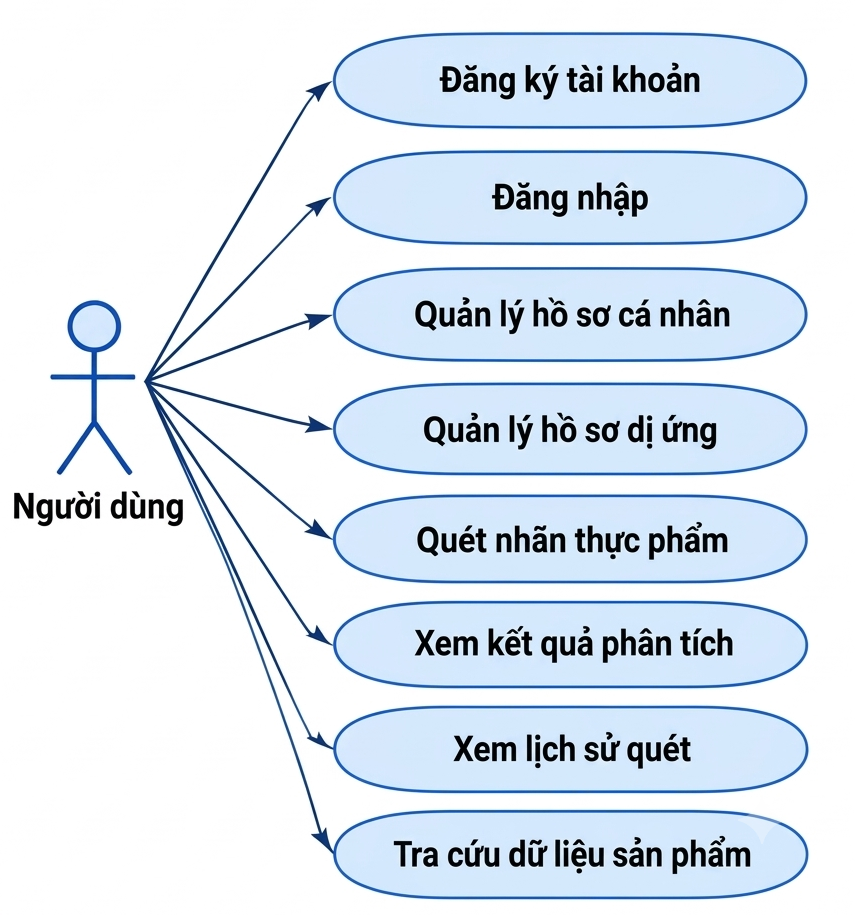
\includegraphics[width=0.82\textwidth,height=0.70\textheight,keepaspectratio]{assets/01_usecase_tongquat.png}
	\caption{Sơ đồ Use Case tổng quát của hệ thống Allergy Warning}
	\label{fig:usecase-tongquat}
\end{figure}

Sơ đồ cho thấy người dùng tương tác với tám nhóm chức năng chính: đăng ký, đăng nhập, quản lý hồ sơ cá nhân, quản lý hồ sơ dị ứng, quét nhãn, xem kết quả, xem lịch sử và tra cứu dữ liệu sản phẩm.


\Needspace{9\baselineskip}
\subsection{Sơ đồ Use Case phân rã chức năng tài khoản}

Nhóm chức năng tài khoản cho phép người dùng tạo tài khoản và xác thực trước khi sử dụng những chức năng yêu cầu đăng nhập. Quá trình đăng ký bao gồm nhập thông tin, kiểm tra dữ liệu và tạo tài khoản. Quá trình đăng nhập bao gồm nhập thông tin xác thực và kiểm tra trạng thái tài khoản.

\begin{figure}[H]
	\centering
	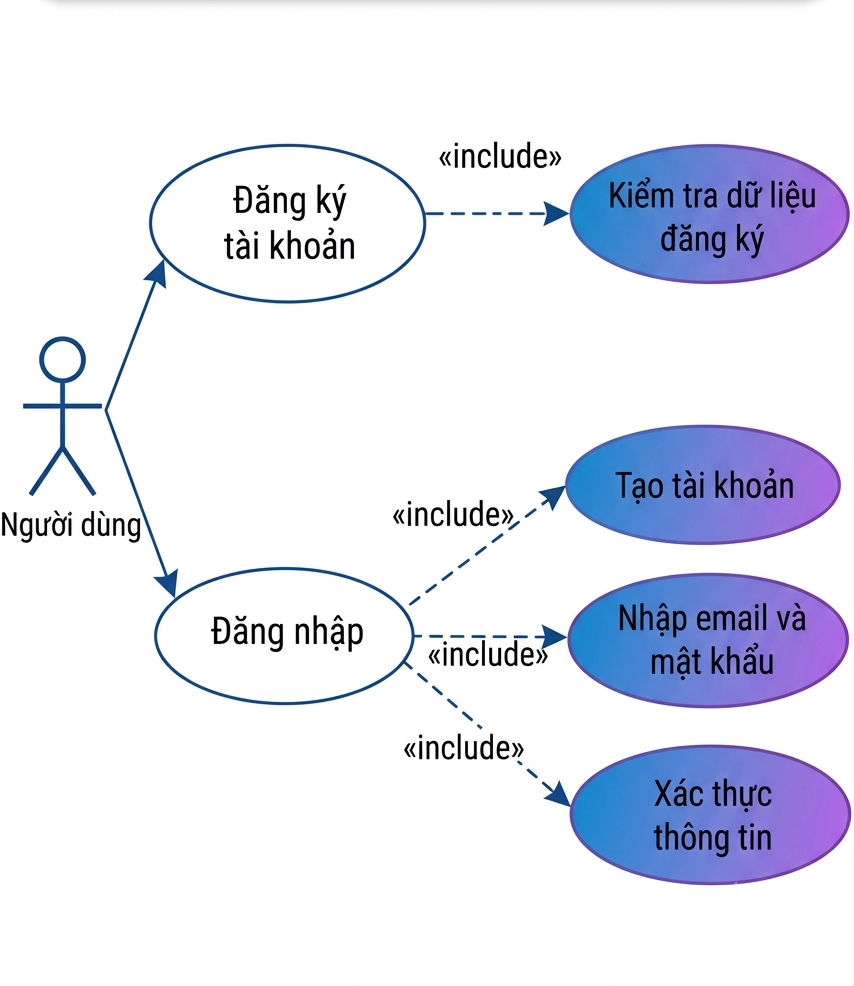
\includegraphics[width=0.82\textwidth,height=0.70\textheight,keepaspectratio]{assets/02_usecase_taikhoan.png}
	\caption{Sơ đồ Use Case phân rã chức năng quản lý tài khoản}
	\label{fig:usecase-taikhoan}
\end{figure}

Sơ đồ phân rã hai chức năng tài khoản. Đăng ký bao gồm kiểm tra dữ liệu trước khi tạo tài khoản; đăng nhập bao gồm nhập email, mật khẩu và xác thực thông tin để cấp quyền truy cập.


\Needspace{9\baselineskip}
\subsection{Sơ đồ Use Case phân rã chức năng quản lý hồ sơ dị ứng}

Chức năng hồ sơ dị ứng cho phép người dùng xem thông tin cá nhân và lựa chọn những nhóm dị nguyên cần chú ý. Danh sách dị nguyên được lấy từ dữ liệu hệ thống. Các lựa chọn của người dùng được liên kết với tài khoản thông qua bảng \texttt{user\_allergens}.

\begin{figure}[H]
	\centering
	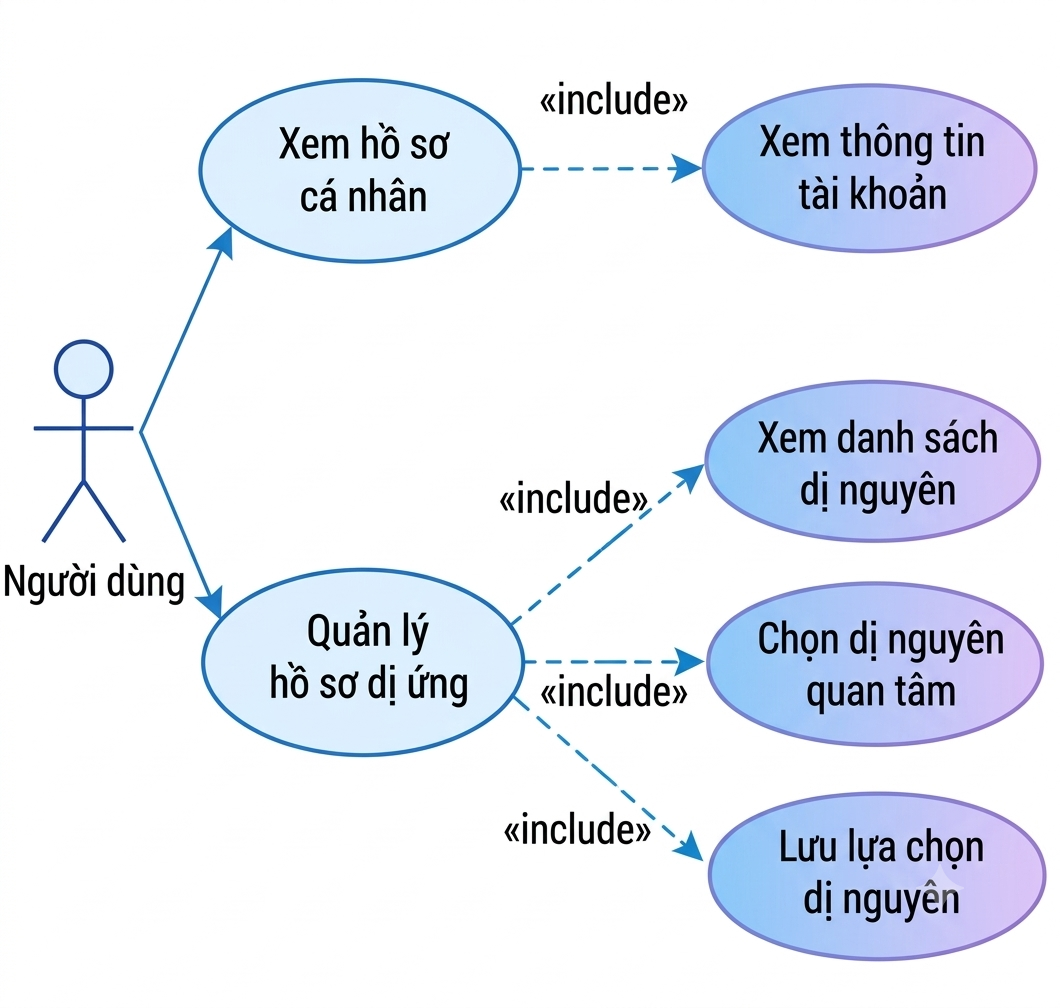
\includegraphics[width=0.82\textwidth,height=0.70\textheight,keepaspectratio]{assets/03_usecase_hoso.png}
	\caption{Sơ đồ Use Case phân rã chức năng quản lý hồ sơ dị ứng}
	\label{fig:usecase-hoso-diung}
\end{figure}

Sơ đồ thể hiện người dùng xem hồ sơ cá nhân và quản lý hồ sơ dị ứng. Với hồ sơ dị ứng, người dùng xem danh sách, chọn các dị nguyên quan tâm và lưu lựa chọn để sử dụng trong những lần phân tích tiếp theo.


\Needspace{9\baselineskip}
\subsection{Sơ đồ Use Case phân rã chức năng quét nhãn thực phẩm}

Quét nhãn thực phẩm là chức năng trọng tâm của hệ thống. Người dùng cung cấp ảnh nhãn, hệ thống kiểm tra ảnh và gửi ảnh đến Gemini API để nhận diện, trích xuất thông tin. Nội dung nhận diện được chuẩn hóa, phân tích thành phần và đối chiếu với dữ liệu dị nguyên. Kết quả được phân loại thành các trường hợp có dị nguyên trong thành phần, có cảnh báo khả năng chứa vết dị nguyên hoặc chưa đủ dữ liệu xác định.

\begin{figure}[H]
	\centering
	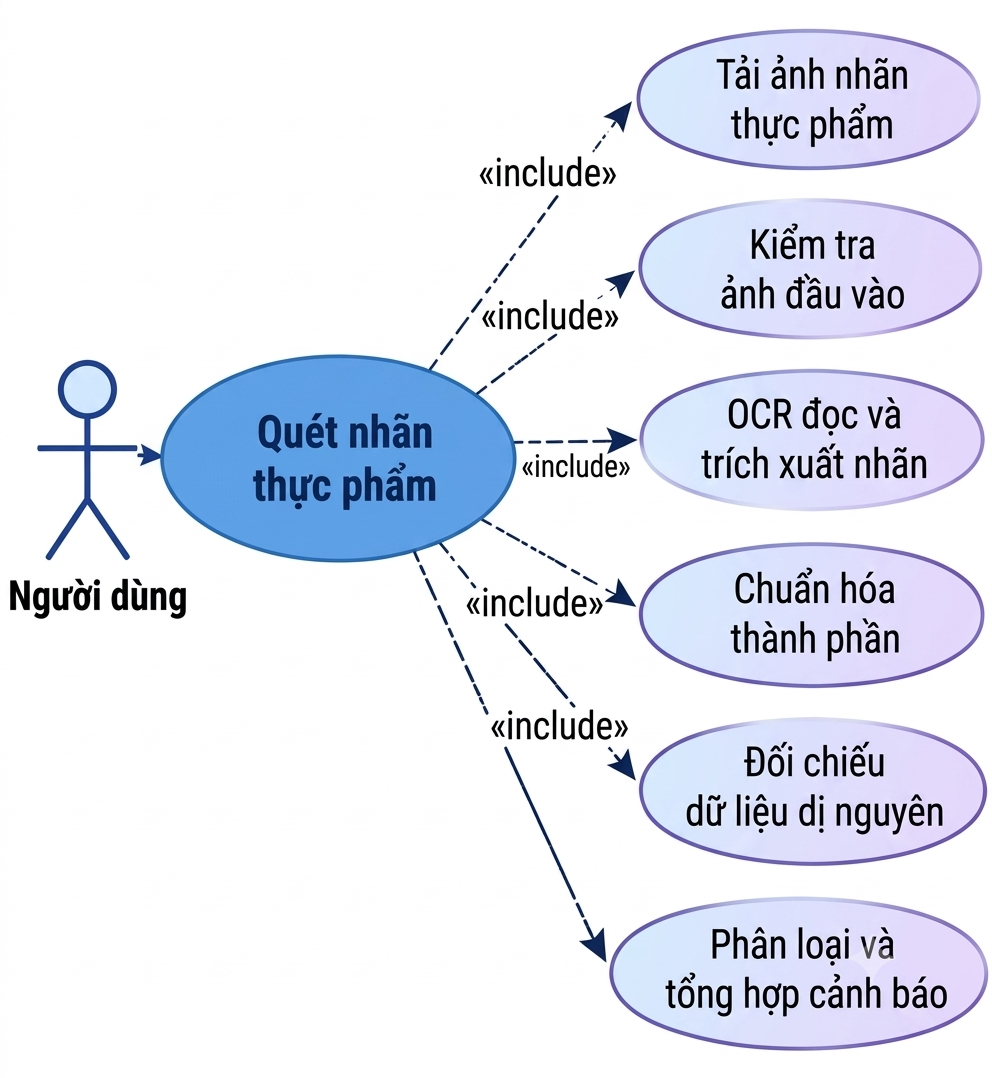
\includegraphics[width=0.92\textwidth,height=0.70\textheight,keepaspectratio]{assets/04_usecase_quetnhan.png}
	\caption{Sơ đồ Use Case phân rã chức năng quét nhãn thực phẩm}
	\label{fig:usecase-quet-nhan}
\end{figure}

Sơ đồ mô tả chức năng quét nhãn và các bước được hệ thống thực hiện: tải ảnh, kiểm tra ảnh đầu vào, dùng OCR/AI trích xuất nội dung, chuẩn hóa thành phần, đối chiếu dữ liệu dị nguyên và tổng hợp cảnh báo.


\Needspace{9\baselineskip}
\subsection{Sơ đồ Use Case phân rã chức năng kết quả và lịch sử}

Sau khi quá trình phân tích hoàn tất, người dùng có thể xem kết quả, theo dõi bằng chứng liên quan đến dị nguyên và tra cứu lại những lần quét trước đó. Dữ liệu lịch sử được truy xuất theo tài khoản đang đăng nhập.

\begin{figure}[H]
	\centering
	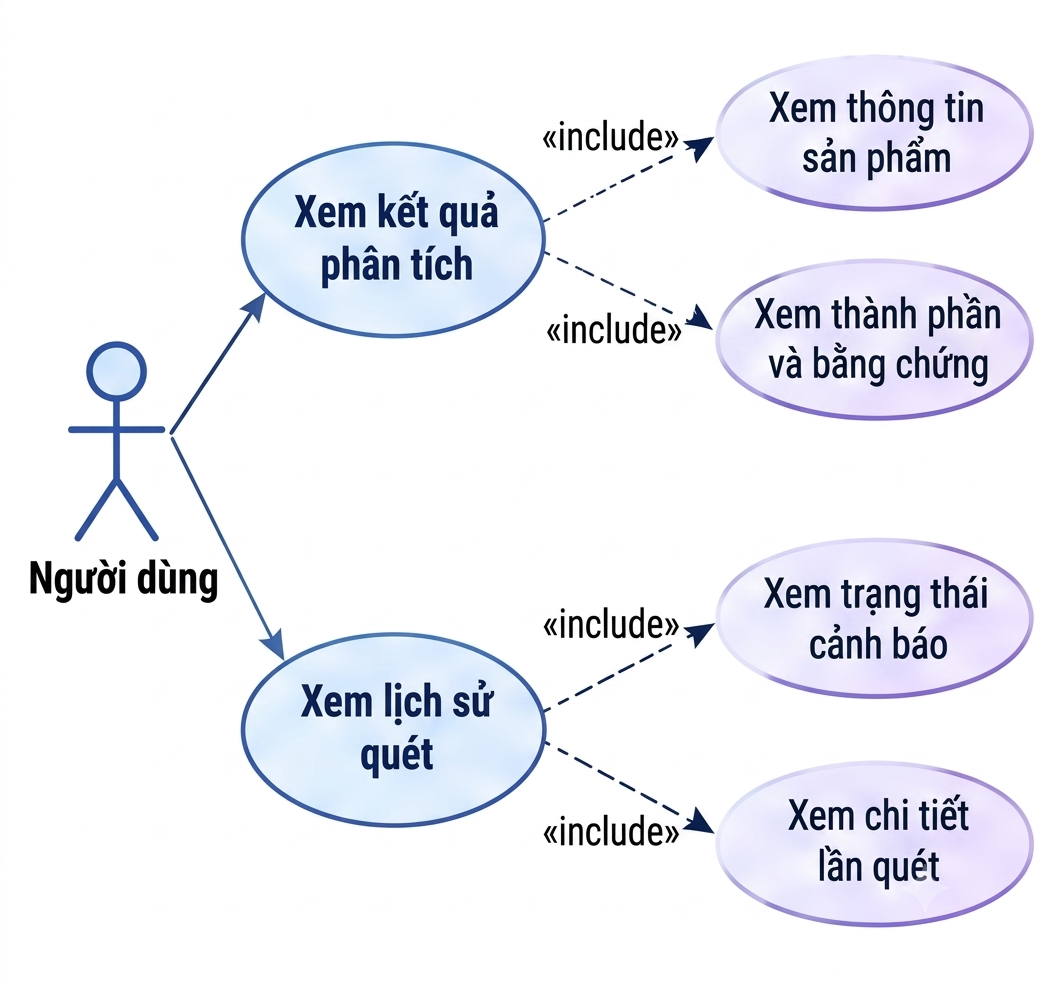
\includegraphics[width=0.82\textwidth,height=0.70\textheight,keepaspectratio]{assets/05_usecase_ketqua.png}
	\caption{Sơ đồ Use Case phân rã chức năng kết quả và lịch sử quét}
	\label{fig:usecase-ketqua-lichsu}
\end{figure}

Sơ đồ thể hiện hai chức năng sau khi quét. Người dùng có thể xem thông tin sản phẩm, thành phần và bằng chứng cảnh báo; đồng thời tra cứu trạng thái và chi tiết của những lần quét đã lưu.


\Needspace{9\baselineskip}
\subsection{Đặc tả các Use Case chính}

Dựa trên các sơ đồ Use Case, những chức năng chính của hệ thống được mô tả tóm tắt trong Bảng~\ref{tab:usecase-description}.

\begin{table}[H]
	\centering
	\caption{Đặc tả các Use Case chính của hệ thống}
	\label{tab:usecase-description}
	\small
	\begin{tabularx}{\textwidth}{|c|l|X|}
		\hline
		\textbf{Mã UC} & \textbf{Tên Use Case} & \textbf{Mô tả chức năng} \\
		\hline
		UC01 & Đăng ký tài khoản & Người dùng nhập họ tên, email và mật khẩu để tạo tài khoản mới. \\
		\hline
		UC02 & Đăng nhập & Người dùng nhập email và mật khẩu để xác thực và truy cập hệ thống. \\
		\hline
		UC03 & Quản lý hồ sơ cá nhân & Người dùng xem thông tin tài khoản của mình. \\
		\hline
		UC04 & Quản lý hồ sơ dị ứng & Người dùng lựa chọn và cập nhật các nhóm dị nguyên cần chú ý. \\
		\hline
		UC05 & Quét nhãn thực phẩm & Người dùng tải ảnh nhãn thực phẩm lên để hệ thống phân tích. \\
		\hline
		UC06 & Xem kết quả phân tích & Người dùng xem thông tin sản phẩm, thành phần và cảnh báo dị nguyên. \\
		\hline
		UC07 & Xem lịch sử quét & Người dùng xem lại những lần quét và kết quả trước đó. \\
		\hline
		UC08 & Quản lý dữ liệu sản phẩm & Quản trị viên tra cứu và quản lý dữ liệu sản phẩm theo quyền được cấp. \\
		\hline
	\end{tabularx}
\end{table}

\Needspace{7\baselineskip}
\subsubsection{Đặc tả Use Case đăng ký tài khoản}

\textbf{Tác nhân:} Người dùng.

\textbf{Mục đích:} Tạo tài khoản mới để sử dụng các chức năng của hệ thống.

\textbf{Điều kiện tiên quyết:} Người dùng chưa có tài khoản sử dụng email đăng ký.

\textbf{Luồng sự kiện chính:}
\begin{enumerate}
	\item Người dùng truy cập trang đăng ký.
	\item Người dùng nhập họ tên, email, mật khẩu và xác nhận mật khẩu.
	\item Hệ thống kiểm tra các trường dữ liệu bắt buộc.
	\item Hệ thống kiểm tra email đã tồn tại hay chưa.
	\item Nếu dữ liệu hợp lệ, hệ thống băm mật khẩu và lưu tài khoản.
	\item Hệ thống thông báo đăng ký thành công.
\end{enumerate}

\textbf{Luồng ngoại lệ:}
\begin{itemize}
	\item Thiếu thông tin: Hệ thống yêu cầu nhập đầy đủ.
	\item Email đã tồn tại: Hệ thống thông báo email đã được sử dụng.
	\item Mật khẩu xác nhận không khớp: Hệ thống yêu cầu kiểm tra lại.
\end{itemize}

\textbf{Điều kiện hậu:} Tài khoản mới được lưu trong cơ sở dữ liệu khi đăng ký thành công.

\Needspace{7\baselineskip}
\subsubsection{Đặc tả Use Case đăng nhập}

\textbf{Tác nhân:} Người dùng.

\textbf{Mục đích:} Xác thực tài khoản để truy cập các chức năng yêu cầu đăng nhập.

\textbf{Điều kiện tiên quyết:} Người dùng đã có tài khoản trong hệ thống.

\textbf{Luồng sự kiện chính:}
\begin{enumerate}
	\item Người dùng mở trang đăng nhập.
	\item Người dùng nhập email và mật khẩu.
	\item Hệ thống kiểm tra thông tin xác thực.
	\item Hệ thống kiểm tra trạng thái hoạt động của tài khoản.
	\item Nếu thông tin hợp lệ, người dùng được chuyển đến trang chính.
\end{enumerate}

\textbf{Luồng ngoại lệ:}
\begin{itemize}
	\item Email hoặc mật khẩu không chính xác: Hệ thống thông báo đăng nhập thất bại.
	\item Tài khoản không hoạt động: Hệ thống từ chối truy cập.
\end{itemize}

\textbf{Điều kiện hậu:} Người dùng được xác thực và có thể truy cập các chức năng phù hợp.

\Needspace{7\baselineskip}
\subsubsection{Đặc tả Use Case quản lý hồ sơ dị ứng}

\textbf{Tác nhân:} Người dùng.

\textbf{Mục đích:} Lưu các nhóm dị nguyên mà người dùng muốn hệ thống chú ý.

\textbf{Điều kiện tiên quyết:} Người dùng đã đăng nhập.

\textbf{Luồng sự kiện chính:}
\begin{enumerate}
	\item Người dùng truy cập trang hồ sơ cá nhân.
	\item Hệ thống hiển thị danh sách các nhóm dị nguyên.
	\item Người dùng lựa chọn hoặc bỏ lựa chọn dị nguyên.
	\item Người dùng xác nhận cập nhật.
	\item Hệ thống lưu lựa chọn vào bảng \texttt{user\_allergens}.
	\item Hệ thống thông báo cập nhật thành công.
\end{enumerate}

\textbf{Luồng ngoại lệ:}
\begin{itemize}
	\item Dữ liệu cập nhật không hợp lệ: Hệ thống yêu cầu kiểm tra lại.
	\item Lỗi lưu dữ liệu: Hệ thống thông báo chưa thể cập nhật hồ sơ.
\end{itemize}

\textbf{Điều kiện hậu:} Hồ sơ dị ứng được cập nhật để sử dụng trong những lần phân tích tiếp theo.

\Needspace{7\baselineskip}
\subsubsection{Đặc tả Use Case quét nhãn thực phẩm}

\textbf{Tác nhân:} Người dùng.

\textbf{Mục đích:} Trích xuất thông tin trên nhãn thực phẩm, đối chiếu thành phần và nhận cảnh báo về các dị nguyên liên quan.

\textbf{Điều kiện tiên quyết:}
\begin{itemize}
	\item Người dùng đã đăng nhập.
	\item Người dùng có ảnh nhãn thực phẩm cần phân tích.
\end{itemize}

\textbf{Luồng sự kiện chính:}
\begin{enumerate}
	\item Người dùng truy cập chức năng quét nhãn.
	\item Người dùng chọn ảnh nhãn từ thiết bị.
	\item Hệ thống tiếp nhận và kiểm tra ảnh đầu vào.
	\item Hệ thống nhận diện và trích xuất thông tin từ ảnh.
	\item Nội dung nhận diện được chuẩn hóa.
	\item Hệ thống đối chiếu thành phần với dữ liệu dị nguyên.
	\item Hệ thống phân loại các trường hợp có dị nguyên trong thành phần, cảnh báo có thể chứa vết dị nguyên hoặc chưa đủ dữ liệu xác định.
	\item Hệ thống tổng hợp thông tin sản phẩm và kết quả cảnh báo.
	\item Kết quả được lưu vào lịch sử quét.
	\item Hệ thống hiển thị kết quả cho người dùng.
\end{enumerate}

\textbf{Luồng ngoại lệ:}
\begin{itemize}
	\item Ảnh không hợp lệ: Hệ thống yêu cầu chọn lại ảnh.
	\item Không nhận diện được nội dung: Hệ thống thông báo không đủ dữ liệu.
	\item Lỗi phân tích: Hệ thống thông báo lỗi và cho phép thực hiện lại.
	\item Không xác định được sản phẩm: Hệ thống vẫn có thể hiển thị kết quả dựa trên nội dung nhận diện được nếu dữ liệu đáp ứng yêu cầu xử lý.
\end{itemize}

\textbf{Điều kiện hậu:} Kết quả được hiển thị và lưu vào lịch sử quét khi quá trình xử lý hoàn thành thành công.

\Needspace{7\baselineskip}
\subsubsection{Đặc tả Use Case xem lịch sử quét}

\textbf{Tác nhân:} Người dùng.

\textbf{Mục đích:} Tra cứu lại những sản phẩm đã được phân tích trước đó.

\textbf{Điều kiện tiên quyết:} Người dùng đã đăng nhập.

\textbf{Luồng sự kiện chính:}
\begin{enumerate}
	\item Người dùng truy cập chức năng lịch sử quét.
	\item Hệ thống xác định tài khoản đang đăng nhập.
	\item Hệ thống truy xuất bản ghi tương ứng trong bảng \texttt{scan\_history}.
	\item Hệ thống hiển thị tên sản phẩm, thời điểm quét và trạng thái cảnh báo.
	\item Người dùng chọn bản ghi để xem chi tiết nếu giao diện hỗ trợ.
\end{enumerate}

\textbf{Luồng ngoại lệ:}
\begin{itemize}
	\item Chưa có lịch sử: Hệ thống thông báo chưa có dữ liệu.
	\item Lỗi truy xuất: Hệ thống thông báo không thể tải lịch sử.
\end{itemize}

\textbf{Điều kiện hậu:} Người dùng xem được các bản ghi lịch sử thuộc tài khoản của mình.

% =========================================================
% 3.4 KIẾN TRÚC HỆ THỐNG
% =========================================================

\Needspace{12\baselineskip}
\section{Thiết kế kiến trúc hệ thống}

\Needspace{9\baselineskip}
\subsection{Kiến trúc tổng thể}

Hệ thống Allergy Warning được tổ chức thành các thành phần chính gồm giao diện web, xử lý nghiệp vụ phía máy chủ, thành phần nhận diện và phân tích nội dung nhãn, cùng cơ sở dữ liệu. Các thành phần phối hợp để tiếp nhận ảnh, xử lý thông tin và trả kết quả cảnh báo cho người dùng.

\begin{figure}[H]
	\centering
	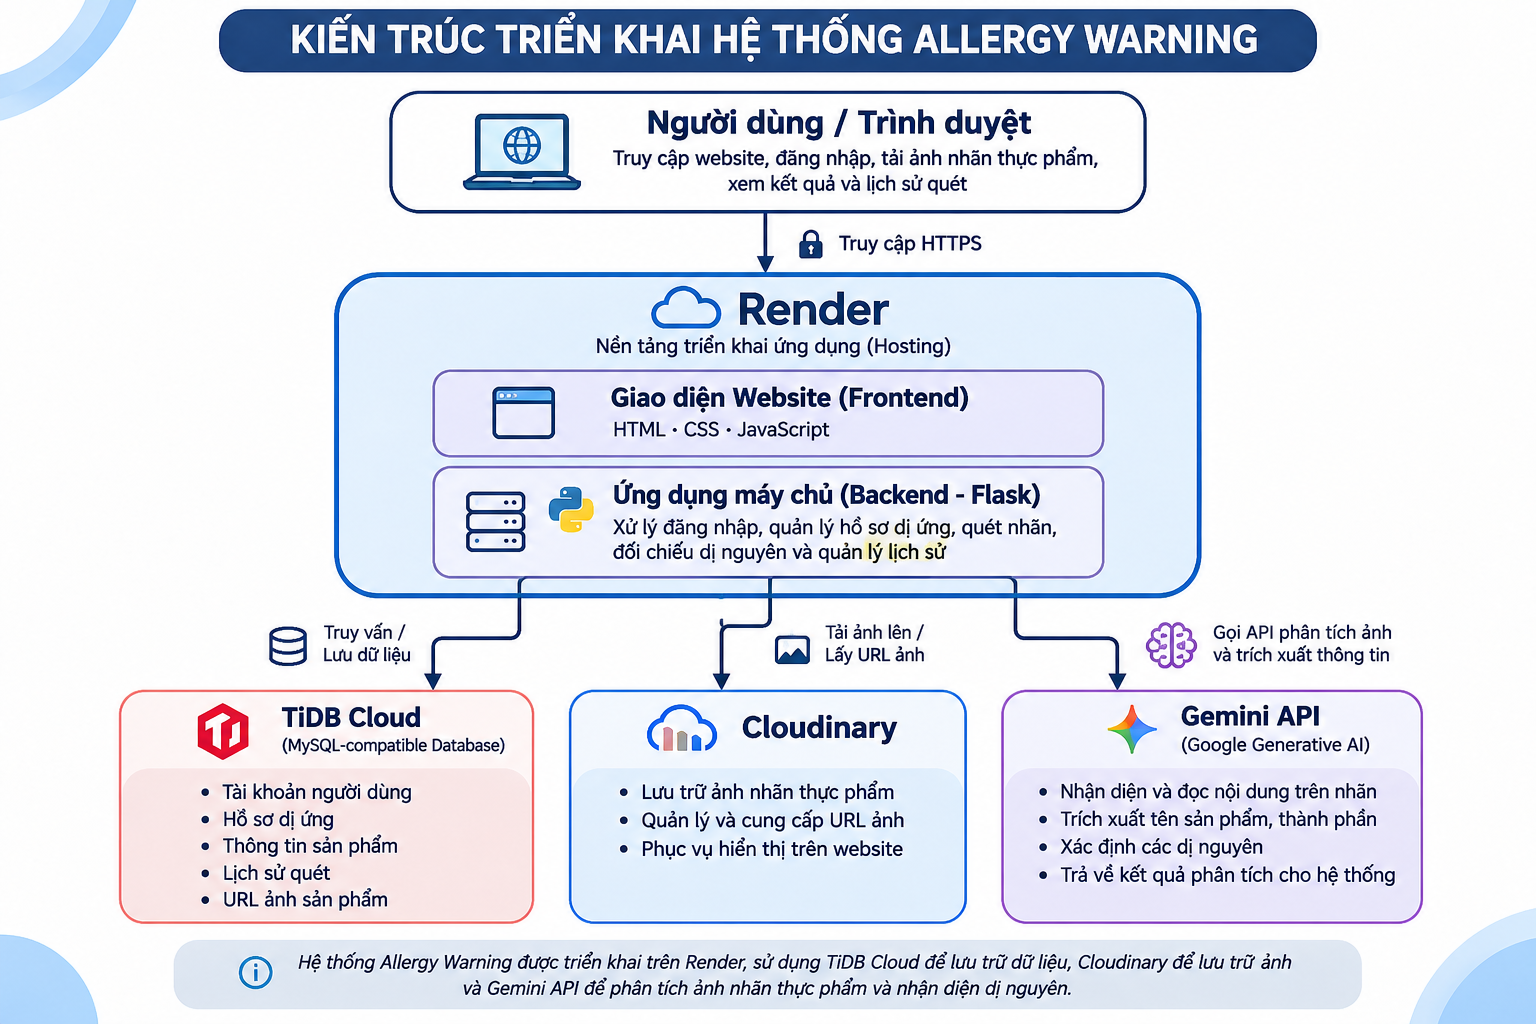
\includegraphics[width=0.95\textwidth,height=0.68\textheight,keepaspectratio]{assets/06_kien_truc_tong_the.png}
	\caption{Kiến trúc tổng thể của hệ thống Allergy Warning}
	\label{fig:kien-truc-he-thong}
\end{figure}

Sơ đồ thể hiện người dùng truy cập website qua HTTPS; ứng dụng Flask được triển khai trên Render, xử lý yêu cầu từ trình duyệt và kết nối các dịch vụ. TiDB Cloud lưu dữ liệu quan hệ, Cloudinary lưu ảnh và cung cấp URL, còn Gemini API phân tích ảnh nhãn và trích xuất thông tin.


\Needspace{9\baselineskip}
\subsection{Sơ đồ kiến trúc xử lý ảnh và phân tích dị nguyên}

Bên cạnh kiến trúc tổng thể, quy trình xử lý nhãn thực phẩm được chia thành các công đoạn. Ảnh đầu vào được tiếp nhận và kiểm tra tính hợp lệ, sau đó được gửi đến Gemini API để nhận diện nội dung hình ảnh và trích xuất thông tin dạng văn bản. Ứng dụng tiếp tục chuẩn hóa kết quả, phân tích tên sản phẩm, thương hiệu, thành phần và các cụm từ cảnh báo. Những thông tin thu được được đối chiếu với dữ liệu dị nguyên để tổng hợp cảnh báo và lưu trữ.

\begin{figure}[H]
	\centering
	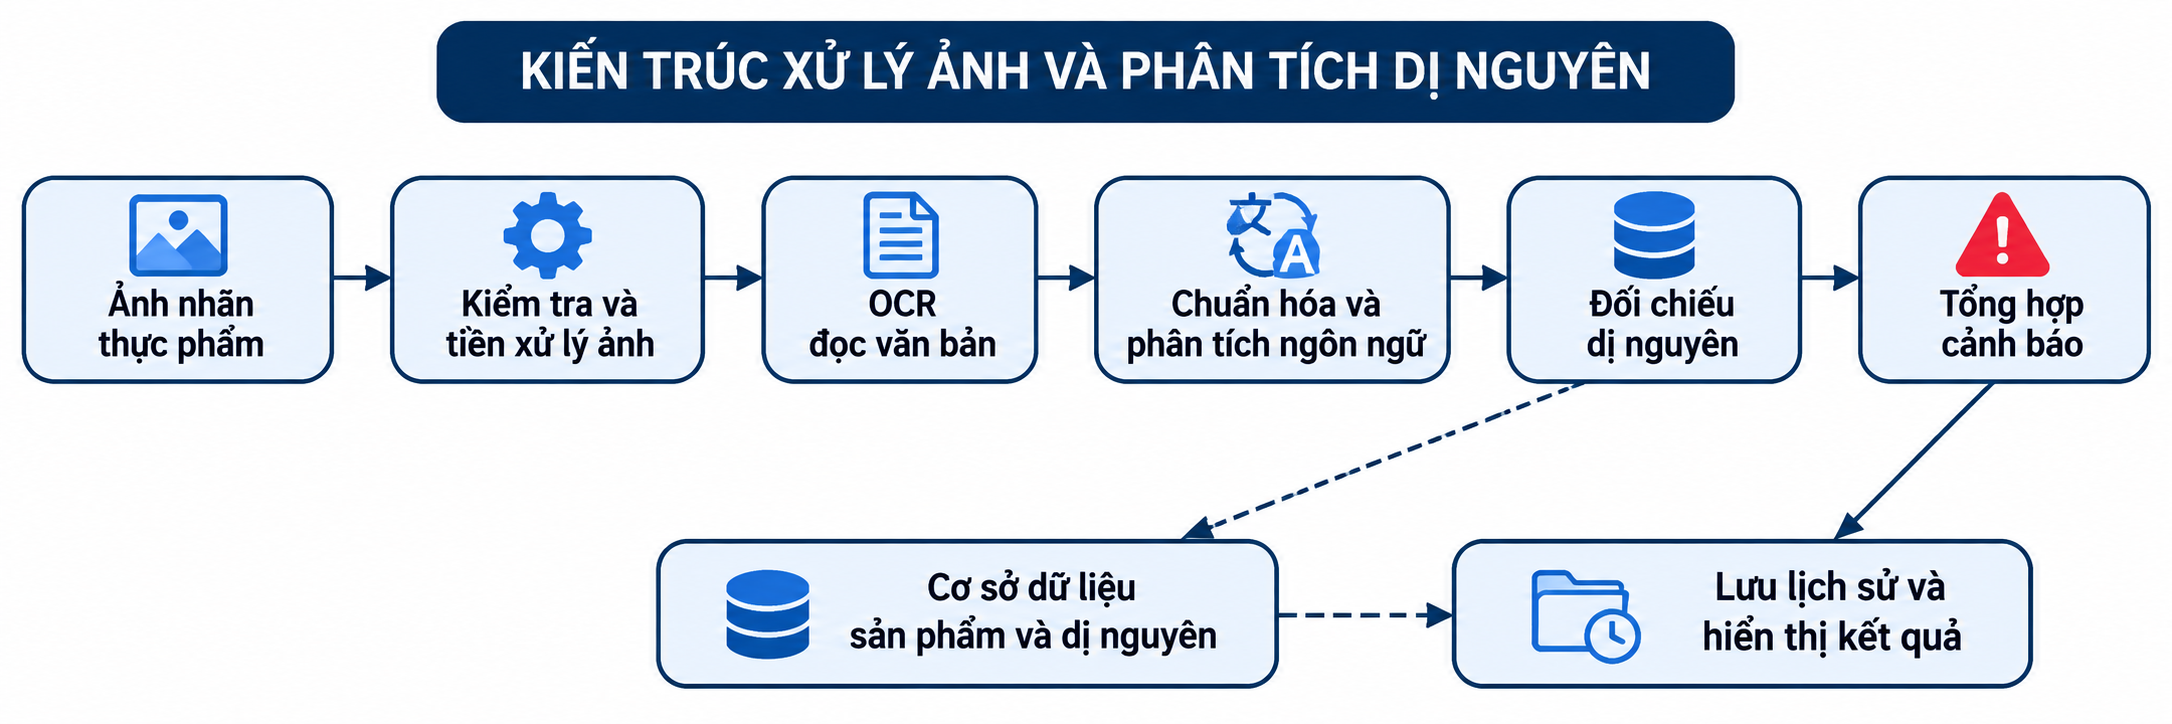
\includegraphics[width=0.95\textwidth,height=0.68\textheight,keepaspectratio]{assets/07_kien_truc_xu_ly.png}
	\caption{Kiến trúc xử lý ảnh và phân tích dị nguyên}
	\label{fig:kien-truc-xu-ly}
\end{figure}

Sơ đồ mô tả chuỗi xử lý ảnh: tiếp nhận ảnh, kiểm tra và tiền xử lý, OCR/AI đọc nội dung, chuẩn hóa ngôn ngữ, đối chiếu dị nguyên, tổng hợp cảnh báo, sau đó lưu lịch sử và hiển thị kết quả.


\Needspace{9\baselineskip}
\subsection{Giao diện web}

Giao diện web là nơi người dùng thực hiện các thao tác với hệ thống. Các trang chính được thể hiện qua những màn hình đăng nhập, đăng ký, Dashboard, quét nhãn, hồ sơ cá nhân, lịch sử quét và kết quả phân tích.

Giao diện sử dụng màu xanh lá làm màu nhấn, nền sáng và các thẻ nội dung riêng biệt. Cách trình bày này giúp phân chia rõ khu vực tải ảnh, danh sách dị nguyên và kết quả cảnh báo.

\Needspace{9\baselineskip}
\subsection{Thành phần xử lý nghiệp vụ}

Thành phần xử lý nghiệp vụ phía máy chủ được xây dựng bằng Flask. Thành phần này tiếp nhận yêu cầu từ giao diện web, kiểm tra dữ liệu đầu vào, điều phối quá trình phân tích ảnh, xử lý kết quả trả về, quản lý tài khoản, truy xuất dữ liệu sản phẩm và lưu lịch sử quét. Máy chủ cũng thực hiện việc kết nối đến các dịch vụ bên ngoài theo cấu hình của hệ thống.

\Needspace{9\baselineskip}
\subsection{Thành phần nhận diện thông tin nhãn}

Thành phần nhận diện sử dụng Gemini API để phân tích ảnh nhãn thực phẩm và trích xuất nội dung có liên quan. Kết quả nhận diện có thể chứa tên sản phẩm, thương hiệu, danh sách thành phần và thông tin cảnh báo được ghi trên bao bì.

Do ảnh đầu vào có thể chứa nhiều ngôn ngữ và bố cục khác nhau, nội dung do mô hình trả về cần được kiểm tra, chuẩn hóa và xử lý trong ứng dụng trước khi chuyển sang bước đối chiếu dị nguyên.

\Needspace{9\baselineskip}
\subsection{Thành phần phân tích và cảnh báo}

Thành phần phân tích sử dụng nội dung nhận diện được và dữ liệu dị nguyên để xác định những thành phần cần chú ý. Kết quả được tổng hợp thành danh sách dị nguyên, thông tin bằng chứng và trạng thái cảnh báo.

Trong giao diện kết quả, hệ thống phân biệt thông tin có bằng chứng từ thành phần với cảnh báo có thể chứa vết dị nguyên. Việc phân biệt này giúp người dùng hiểu rõ hơn căn cứ của từng cảnh báo.

\Needspace{9\baselineskip}
\subsection{Thành phần cơ sở dữ liệu}

Cơ sở dữ liệu được thiết kế theo mô hình quan hệ và sử dụng hệ quản trị tương thích MySQL. Trong môi trường phát triển, hệ thống có thể kết nối MySQL/MariaDB cục bộ; khi triển khai trực tuyến, ứng dụng sử dụng TiDB Cloud theo thông tin kết nối được cấu hình. Cơ sở dữ liệu lưu thông tin tài khoản, dị nguyên, sản phẩm, thành phần sản phẩm, hồ sơ dị ứng và lịch sử quét.

Cơ sở dữ liệu gồm sáu bảng chính: \texttt{user}, \texttt{allergens}, \texttt{products}, \texttt{product\_ingredients}, \texttt{user\_allergens} và \texttt{scan\_history}.

\Needspace{9\baselineskip}
\subsection{Dịch vụ bên ngoài}

\textbf{Gemini API:} Được sử dụng để hỗ trợ phân tích ảnh nhãn thực phẩm và trích xuất thông tin như tên sản phẩm, thương hiệu, thành phần và nội dung cảnh báo. Kết quả do mô hình trả về tiếp tục được ứng dụng kiểm tra và xử lý trước khi hiển thị.

\textbf{Cloudinary:} Được sử dụng để lưu trữ ảnh được tải lên theo cấu hình của hệ thống. Sau khi tải ảnh thành công, ứng dụng nhận đường dẫn ảnh và có thể lưu đường dẫn này trong dữ liệu lịch sử quét để phục vụ việc hiển thị lại.

\textbf{TiDB Cloud:} Là dịch vụ cơ sở dữ liệu được sử dụng trong môi trường triển khai trực tuyến. Ứng dụng kết nối đến cơ sở dữ liệu thông qua các thông số kết nối được cấu hình trong biến môi trường.

Các dịch vụ trên đảm nhiệm những vai trò khác nhau: Gemini API hỗ trợ phân tích nội dung ảnh, Cloudinary lưu trữ ảnh, còn TiDB Cloud lưu trữ dữ liệu có cấu trúc của hệ thống.

% =========================================================
% 3.5 THIẾT KẾ QUY TRÌNH
% =========================================================

\Needspace{12\baselineskip}
\section{Thiết kế quy trình xử lý}

\Needspace{9\baselineskip}
\subsection{Quy trình đăng ký và đăng nhập}

Đối với người dùng mới, hệ thống tiếp nhận thông tin đăng ký và kiểm tra các trường bắt buộc. Khi dữ liệu hợp lệ, thông tin tài khoản được lưu trong bảng \texttt{user}.

Khi đăng nhập, hệ thống tiếp nhận email và mật khẩu, thực hiện xác thực và kiểm tra trạng thái tài khoản. Sau khi xác thực thành công, người dùng có thể truy cập những chức năng yêu cầu đăng nhập.

\Needspace{9\baselineskip}
\subsection{Quy trình quản lý hồ sơ dị ứng}

Người dùng truy cập trang hồ sơ cá nhân và lựa chọn các nhóm dị nguyên cần chú ý. Các lựa chọn được liên kết với tài khoản thông qua bảng \texttt{user\_allergens}.

Khi người dùng thay đổi lựa chọn, hệ thống cần cập nhật dữ liệu tương ứng để các lần phân tích sau có thể sử dụng hồ sơ dị ứng mới nhất.

\Needspace{9\baselineskip}
\subsection{Quy trình quét nhãn thực phẩm}

Quy trình quét nhãn được thực hiện theo các bước sau:

\textbf{Bước 1: Chọn ảnh nhãn thực phẩm.}

Người dùng truy cập chức năng quét nhãn, chọn ảnh từ thiết bị và kiểm tra tên ảnh đã chọn trên giao diện.

\textbf{Bước 2: Gửi ảnh lên hệ thống.}

Ảnh được gửi đến ứng dụng phía máy chủ để tiếp nhận và xử lý. Hệ thống cần kiểm tra dữ liệu đầu vào trước khi thực hiện phân tích.

\textbf{Bước 3: Nhận diện thông tin.}

Ứng dụng gửi ảnh đến Gemini API để phân tích và trích xuất thông tin có thể nhận diện, bao gồm tên sản phẩm, thương hiệu, nội dung thành phần và thông tin cảnh báo trên nhãn.

\textbf{Bước 4: Chuẩn hóa nội dung.}

Nội dung do Gemini API trả về được ứng dụng xử lý để thuận tiện cho việc phân tích. Quá trình này có thể bao gồm chuẩn hóa chữ hoa, chữ thường, khoảng trắng và các cách viết của tên thành phần.

\textbf{Bước 5: Đối chiếu dị nguyên.}

Hệ thống đối chiếu thông tin thành phần và dữ liệu dị nguyên. Những nội dung phù hợp với quy tắc đối chiếu được ghi nhận để tạo kết quả cảnh báo.

\textbf{Bước 6: Tổng hợp kết quả.}

Hệ thống tổng hợp tên sản phẩm, thương hiệu, thành phần, dị nguyên và bằng chứng liên quan. Trạng thái cảnh báo được xác định theo kết quả xử lý.

\textbf{Bước 7: Lưu lịch sử quét.}

Kết quả được lưu trong bảng \texttt{scan\_history} cùng mã người dùng và thời điểm thực hiện.

\textbf{Bước 8: Hiển thị kết quả.}

Giao diện hiển thị nội dung phân tích, các thành phần được nhận diện và cảnh báo tương ứng để người dùng theo dõi.

\Needspace{9\baselineskip}
\subsection{Sơ đồ hoạt động quy trình quét nhãn}

Sơ đồ hoạt động mô tả trình tự xử lý từ khi người dùng chọn ảnh đến khi nhận được kết quả. Sơ đồ thể hiện các nhánh kiểm tra ảnh hợp lệ, khả năng nhận diện nội dung và việc tổng hợp cảnh báo. Nếu ảnh không hợp lệ hoặc không đủ thông tin, hệ thống thông báo cho người dùng thay vì đưa ra kết luận không có dị nguyên.

\begin{figure}[H]
	\centering
	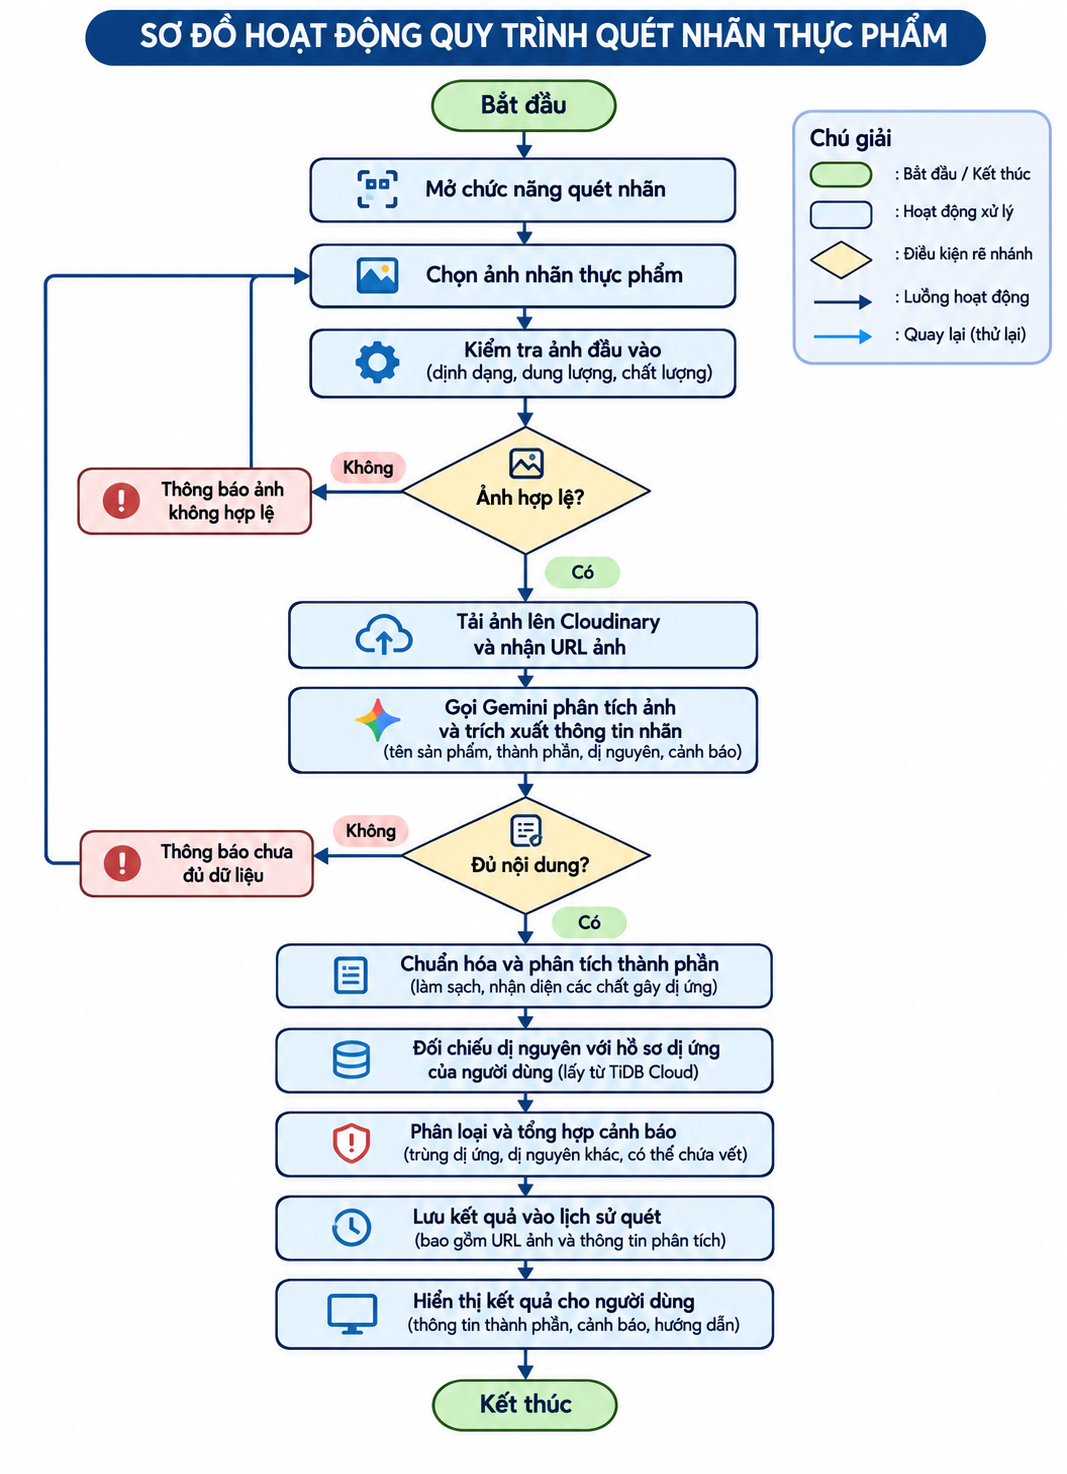
\includegraphics[width=0.72\textwidth,height=0.78\textheight,keepaspectratio]{assets/08_activity_quetnhan.png}
	\caption{Sơ đồ hoạt động quy trình quét nhãn thực phẩm}
	\label{fig:activity-quet-nhan}
\end{figure}

Sơ đồ hoạt động thể hiện luồng xử lý và hai nhánh kiểm tra. Ảnh không hợp lệ hoặc nội dung nhận diện chưa đủ sẽ được thông báo để người dùng thử lại; chỉ khi dữ liệu đạt yêu cầu, hệ thống mới chuẩn hóa, đối chiếu dị nguyên, lưu lịch sử và hiển thị kết quả.


\Needspace{9\baselineskip}
\subsection{Sơ đồ tuần tự quy trình quét nhãn}

Sơ đồ tuần tự mô tả sự trao đổi thông tin giữa người dùng, giao diện web, ứng dụng xử lý nghiệp vụ, thành phần nhận diện và phân tích, cùng cơ sở dữ liệu. Người dùng gửi ảnh từ giao diện; máy chủ tiếp nhận và điều phối quá trình nhận diện, đối chiếu dị nguyên, lưu kết quả rồi trả thông tin phân tích về giao diện.

\begin{figure}[H]
	\centering
	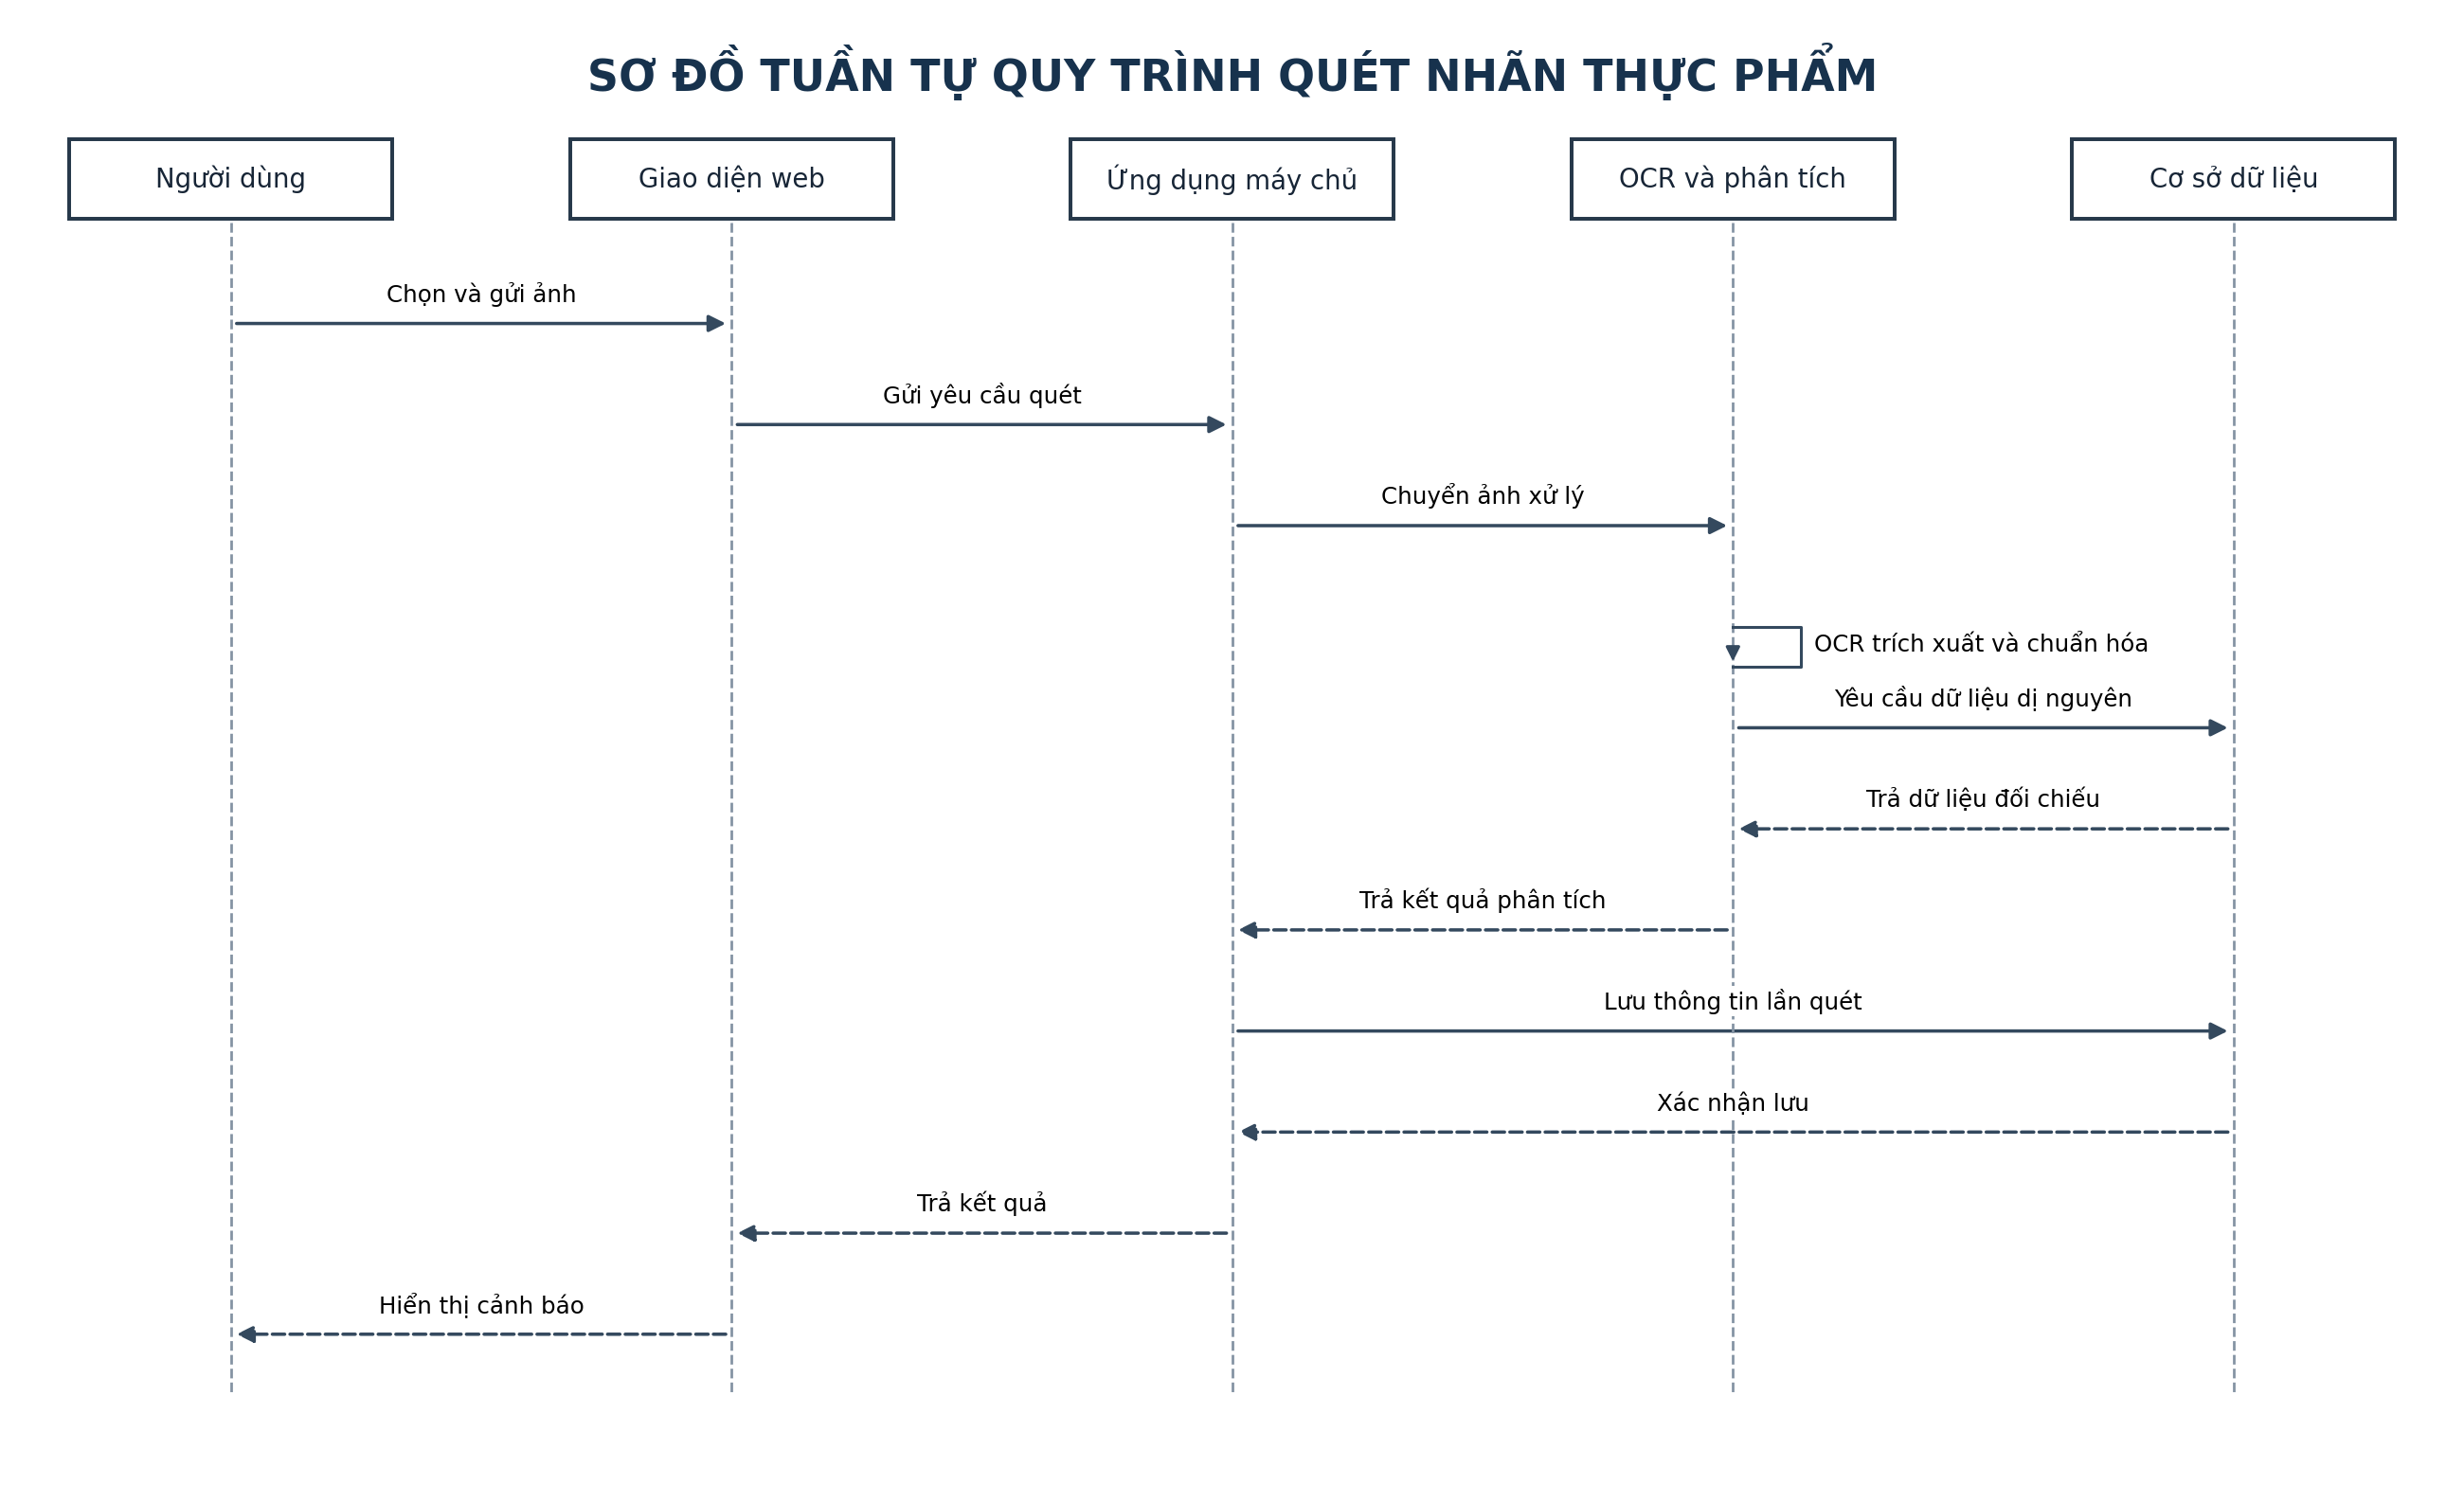
\includegraphics[width=0.95\textwidth,height=0.68\textheight,keepaspectratio]{assets/09_sequence_quetnhan.png}
	\caption{Sơ đồ tuần tự quy trình quét nhãn thực phẩm}
	\label{fig:sequence-quet-nhan}
\end{figure}

Sơ đồ tuần tự mô tả thứ tự trao đổi giữa người dùng, giao diện web, máy chủ, thành phần OCR/phân tích và cơ sở dữ liệu. Máy chủ nhận ảnh, chuyển xử lý, yêu cầu dữ liệu dị nguyên, nhận kết quả, lưu lần quét rồi trả kết quả để giao diện hiển thị cảnh báo.


\Needspace{9\baselineskip}
\subsection{Quy trình phân loại cảnh báo}

Hệ thống cần phân biệt ít nhất hai nhóm thông tin trong kết quả phân tích.

\textbf{Trường hợp thứ nhất: Dị nguyên có bằng chứng trong thành phần.}

Trường hợp này xảy ra khi thông tin thành phần hoặc dữ liệu sản phẩm có nội dung liên quan đến dị nguyên theo quy tắc đối chiếu. Hệ thống hiển thị tên dị nguyên và bằng chứng tương ứng.

\textbf{Trường hợp thứ hai: Cảnh báo có thể chứa vết dị nguyên.}

Trường hợp này được sử dụng khi nhãn có nội dung cảnh báo về khả năng chứa vết dị nguyên nhưng chưa có bằng chứng xác định chắc chắn dị nguyên đó là thành phần thực sự của sản phẩm.

\textbf{Trường hợp thứ ba: Chưa xác định được kết quả.}

Khi dữ liệu đầu vào không đủ hoặc quá trình nhận diện không thu được thông tin cần thiết, hệ thống cần thông báo trạng thái chưa xác định thay vì khẳng định sản phẩm không chứa dị nguyên.

\Needspace{9\baselineskip}
\subsection{Quy trình xem lịch sử quét}

Người dùng truy cập trang lịch sử quét để xem các lần phân tích trước đó. Hệ thống truy xuất những bản ghi liên quan đến tài khoản và hiển thị tên sản phẩm, hình ảnh, thời điểm quét cùng trạng thái cảnh báo.

Việc liên kết lịch sử với tài khoản giúp phân biệt dữ liệu của từng người dùng và hỗ trợ tra cứu lại kết quả đã thực hiện.

% =========================================================
% 3.6 THIẾT KẾ CƠ SỞ DỮ LIỆU
% =========================================================

\Needspace{12\baselineskip}
\section{Thiết kế cơ sở dữ liệu}

\Needspace{9\baselineskip}
\subsection{Mục tiêu thiết kế}

Cơ sở dữ liệu của hệ thống được đặt tên là \texttt{food\_allergen\_system}. Cấu trúc dữ liệu được thiết kế theo mô hình quan hệ, tương thích với MySQL. Trong quá trình phát triển, cơ sở dữ liệu có thể được chạy trên MySQL/MariaDB cục bộ; ở môi trường triển khai trực tuyến, ứng dụng kết nối đến TiDB Cloud. Dữ liệu được chia thành các bảng theo chức năng để quản lý tài khoản, dị nguyên, sản phẩm, thành phần sản phẩm, hồ sơ dị ứng và lịch sử quét.

Việc tách dữ liệu thành các bảng riêng biệt giúp hạn chế lưu trữ trùng lặp, hỗ trợ truy xuất thông tin và xác định mối quan hệ giữa các đối tượng trong hệ thống.

\Needspace{9\baselineskip}
\subsection{Danh sách các bảng dữ liệu}

Cơ sở dữ liệu hiện có sáu bảng chính. Các bảng và trường dưới đây được mô tả theo cấu trúc trong tệp SQL đã cung cấp.

\Needspace{7\baselineskip}
\subsubsection{Bảng allergens}

Bảng \texttt{allergens} lưu danh sách các nhóm dị nguyên được sử dụng trong quá trình đối chiếu.

\begin{table}[H]
	\centering
	\caption{Cấu trúc bảng allergens}
	\label{tab:allergens}
	\small
	\begin{tabularx}{\textwidth}{|l|l|X|l|}
		\hline
		\textbf{Trường} & \textbf{Kiểu dữ liệu} & \textbf{Ý nghĩa} & \textbf{Ràng buộc} \\
		\hline
		id & INT(11) & Mã dị nguyên & Khóa chính, tự tăng \\
		\hline
		name & VARCHAR(100) & Tên dị nguyên bằng tiếng Việt & NOT NULL, UNIQUE \\
		\hline
		description & VARCHAR(255) & Mô tả dị nguyên & Cho phép NULL \\
		\hline
		name\_en & VARCHAR(255) & Tên dị nguyên bằng tiếng Anh & Cho phép NULL \\
		\hline
		off\_tag & VARCHAR(255) & Nhãn dị nguyên theo dữ liệu Open Food Facts & Cho phép NULL \\
		\hline
		created\_at & DATETIME & Thời điểm tạo bản ghi & Mặc định thời gian hiện tại \\
		\hline
	\end{tabularx}
\end{table}

Trường \texttt{id} xác định duy nhất mỗi dị nguyên. Trường \texttt{name} lưu tên hiển thị trên giao diện, còn \texttt{name\_en} và \texttt{off\_tag} hỗ trợ đối chiếu với dữ liệu sản phẩm sử dụng tên tiếng Anh hoặc nhãn chuẩn hóa.

\Needspace{7\baselineskip}
\subsubsection{Bảng products}

Bảng \texttt{products} lưu thông tin sản phẩm thực phẩm đã được thu thập hoặc bổ sung vào hệ thống.

\begin{table}[H]
	\centering
	\caption{Cấu trúc bảng products}
	\label{tab:products}
	\small
	\begin{tabularx}{\textwidth}{|l|l|X|l|}
		\hline
		\textbf{Trường} & \textbf{Kiểu dữ liệu} & \textbf{Ý nghĩa} & \textbf{Ràng buộc} \\
		\hline
		id & INT(11) & Mã sản phẩm & Khóa chính, tự tăng \\
		\hline
		barcode & VARCHAR(50) & Mã vạch sản phẩm & UNIQUE, cho phép NULL \\
		\hline
		name & VARCHAR(255) & Tên sản phẩm & NOT NULL \\
		\hline
		brand & VARCHAR(255) & Thương hiệu sản phẩm & Cho phép NULL \\
		\hline
		ingredients\_text & TEXT & Văn bản thành phần sản phẩm & Cho phép NULL \\
		\hline
		allergens\_text & TEXT & Thông tin dị nguyên được khai báo & Cho phép NULL \\
		\hline
		allergens\_tags & TEXT & Danh sách nhãn dị nguyên & Cho phép NULL \\
		\hline
		image\_url & VARCHAR(1000) & Đường dẫn ảnh sản phẩm & Cho phép NULL \\
		\hline
		source\_url & VARCHAR(1000) & Đường dẫn nguồn dữ liệu & Cho phép NULL \\
		\hline
		created\_at & DATETIME & Thời điểm tạo bản ghi & Mặc định thời gian hiện tại \\
		\hline
	\end{tabularx}
\end{table}

Bảng \texttt{products} lưu các thông tin cơ bản của sản phẩm. Trường \texttt{ingredients\_\allowbreak text} chứa nội dung thành phần dạng văn bản, còn \texttt{allergens\_\allowbreak text} và \texttt{allergens\_\allowbreak tags} lưu thông tin dị nguyên được khai báo. Trường \texttt{image\_\allowbreak url} có thể lưu đường dẫn ảnh sản phẩm và \texttt{source\_\allowbreak url} lưu địa chỉ nguồn dữ liệu khi có.

\Needspace{7\baselineskip}
\subsubsection{Bảng product\_ingredients}

Bảng \texttt{product\_ingredients} lưu từng thành phần của sản phẩm, giúp hệ thống quản lý thành phần dưới dạng các bản ghi riêng.

\begin{table}[H]
	\centering
	\caption{Cấu trúc bảng product\_ingredients}
	\label{tab:product-ingredients}
	\small
	\begin{tabularx}{\textwidth}{|l|l|X|l|}
		\hline
		\textbf{Trường} & \textbf{Kiểu dữ liệu} & \textbf{Ý nghĩa} & \textbf{Ràng buộc} \\
		\hline
		id & INT(11) & Mã thành phần & Khóa chính, tự tăng \\
		\hline
		product\_id & INT(11) & Mã sản phẩm chứa thành phần & Khóa ngoại \\
		\hline
		name & VARCHAR(255) & Tên thành phần & NOT NULL \\
		\hline
		name\_en & VARCHAR(255) & Tên tiếng Anh của thành phần & Cho phép NULL \\
		\hline
		off\_tag & VARCHAR(255) & Nhãn thành phần theo Open Food Facts & Cho phép NULL \\
		\hline
	\end{tabularx}
\end{table}

Trường \texttt{product\_id} liên kết thành phần với bảng \texttt{products}. Khi một sản phẩm có nhiều thành phần, mỗi thành phần được lưu thành một bản ghi riêng. Ràng buộc khóa ngoại được thiết lập để bảo đảm thành phần tham chiếu đến sản phẩm hợp lệ.

\Needspace{7\baselineskip}
\subsubsection{Bảng user}

Bảng \texttt{user} lưu thông tin tài khoản người dùng và trạng thái tài khoản trong hệ thống.

\begin{table}[H]
	\centering
	\caption{Cấu trúc bảng user}
	\label{tab:user}
	\small
	\begin{tabularx}{\textwidth}{|l|l|X|l|}
		\hline
		\textbf{Trường} & \textbf{Kiểu dữ liệu} & \textbf{Ý nghĩa} & \textbf{Ràng buộc} \\
		\hline
		id & CHAR(32) & Mã định danh người dùng & Khóa chính \\
		\hline
		email & VARCHAR(255) & Email đăng nhập & NOT NULL, UNIQUE \\
		\hline
		full\_name & VARCHAR(255) & Họ và tên người dùng & Cho phép NULL \\
		\hline
		hashed\_password & VARCHAR(255) & Giá trị băm của mật khẩu & NOT NULL \\
		\hline
		is\_active & TINYINT(1) & Trạng thái hoạt động của tài khoản & NOT NULL \\
		\hline
		is\_superuser & TINYINT(1) & Xác định tài khoản quản trị & NOT NULL \\
		\hline
		created\_at & DATETIME & Thời điểm tạo tài khoản & Cho phép NULL \\
		\hline
	\end{tabularx}
\end{table}

Trường \texttt{id} dùng để định danh tài khoản. Trường \texttt{email} có ràng buộc duy nhất nhằm hạn chế tạo nhiều tài khoản cùng email. Trường \texttt{hashed\_password} lưu giá trị băm mật khẩu, không lưu mật khẩu ở dạng văn bản thông thường. Hai trường \texttt{is\_active} và \texttt{is\_superuser} thể hiện trạng thái hoạt động và quyền quản trị của tài khoản.

\Needspace{7\baselineskip}
\subsubsection{Bảng user\_allergens}

Bảng \texttt{user\_allergens} liên kết người dùng với các nhóm dị nguyên mà họ lựa chọn trong hồ sơ cá nhân.

\begin{table}[H]
	\centering
	\caption{Cấu trúc bảng user\_allergens}
	\label{tab:user-allergens}
	\small
	\begin{tabularx}{\textwidth}{|l|l|X|l|}
		\hline
		\textbf{Trường} & \textbf{Kiểu dữ liệu} & \textbf{Ý nghĩa} & \textbf{Ràng buộc} \\
		\hline
		id & INT(11) & Mã bản ghi hồ sơ dị ứng & Khóa chính, tự tăng \\
		\hline
		user\_id & CHAR(32) & Mã người dùng & Khóa ngoại \\
		\hline
		allergen\_id & INT(11) & Mã dị nguyên được lựa chọn & Khóa ngoại \\
		\hline
		created\_at & DATETIME & Thời điểm thêm dị nguyên & Mặc định thời gian hiện tại \\
		\hline
	\end{tabularx}
\end{table}

Trường \texttt{user\_id} liên kết với bảng \texttt{user}, còn \texttt{allergen\_id} liên kết với bảng \texttt{allergens}. Cặp trường \texttt{user\_id} và \texttt{allergen\_id} có ràng buộc duy nhất kết hợp, nhằm tránh lưu trùng cùng một dị nguyên cho một người dùng.

\Needspace{7\baselineskip}
\subsubsection{Bảng scan\_history}

Bảng \texttt{scan\_history} lưu lịch sử phân tích nhãn thực phẩm của người dùng.

\begin{table}[H]
	\centering
	\caption{Cấu trúc bảng scan\_history}
	\label{tab:scan-history}
	\scriptsize
	\begin{tabularx}{\textwidth}{|l|l|X|l|}
		\hline
		\textbf{Trường} & \textbf{Kiểu dữ liệu} & \textbf{Ý nghĩa} & \textbf{Ràng buộc} \\
		\hline
		id & INT(11) & Mã bản ghi lịch sử & Khóa chính, tự tăng \\
		\hline
		scan\_id & VARCHAR(32) & Mã định danh lần quét & NOT NULL, UNIQUE \\
		\hline
		user\_id & CHAR(32) & Người thực hiện quét & Khóa ngoại, NOT NULL \\
		\hline
		product\_id & INT(11) & Mã sản phẩm liên quan nếu xác định được & Khóa ngoại, cho phép NULL \\
		\hline
		product\_name & VARCHAR(255) & Tên sản phẩm được nhận diện & NOT NULL \\
		\hline
		brand & VARCHAR(255) & Thương hiệu sản phẩm & Cho phép NULL \\
		\hline
		image\_url & VARCHAR(1000) & Đường dẫn ảnh đã tải lên & Cho phép NULL \\
		\hline
		ingredients\_json & TEXT & Danh sách thành phần ở dạng JSON & NOT NULL \\
		\hline
		allergens\_json & TEXT & Danh sách dị nguyên ở dạng JSON & NOT NULL \\
		\hline
		warnings\_json & TEXT & Chi tiết cảnh báo ở dạng JSON & NOT NULL \\
		\hline
		warning\_status & VARCHAR(20) & Trạng thái cảnh báo & NOT NULL \\
		\hline
		scanned\_at & DATETIME & Thời điểm thực hiện quét & NOT NULL, mặc định thời gian hiện tại \\
		\hline
	\end{tabularx}
\end{table}

Bảng \texttt{scan\_history} lưu kết quả của từng lần quét. Các trường \texttt{ingredients\_json}, \texttt{allergens\_json} và \texttt{warnings\_json} lưu dữ liệu có cấu trúc JSON dưới dạng văn bản. Cách tổ chức này cho phép lưu danh sách thành phần, dị nguyên và chi tiết cảnh báo của từng lần phân tích.

Trường \texttt{warning\_status} thể hiện trạng thái kết quả, còn \texttt{scanned\_at} lưu thời điểm thực hiện. Trường \texttt{product\_id} có thể để trống khi hệ thống chưa xác định được sản phẩm tương ứng.

\Needspace{9\baselineskip}
\subsection{Mối quan hệ giữa các bảng}

Cơ sở dữ liệu sử dụng các khóa chính và khóa ngoại để liên kết sáu bảng. Các quan hệ chính gồm:

\begin{itemize}
	\item \texttt{user} -- \texttt{scan\_history}: quan hệ một-nhiều. Một người dùng có thể thực hiện nhiều lần quét; mỗi bản ghi lịch sử thuộc về một người dùng thông qua \texttt{user\_id}.
	\item \texttt{products} -- \texttt{scan\_history}: quan hệ một-nhiều. Một sản phẩm có thể xuất hiện trong nhiều lần quét. Trường \texttt{product\_id} trong lịch sử cho phép NULL nếu chưa xác định được sản phẩm.
	\item \texttt{products} -- \texttt{product\_ingredients}: quan hệ một-nhiều. Một sản phẩm có thể có nhiều thành phần; mỗi thành phần tham chiếu sản phẩm qua \texttt{product\_id}.
	\item \texttt{user} -- \texttt{user\_allergens}: quan hệ một-nhiều. Một người dùng có thể lưu nhiều dị nguyên quan tâm.
	\item \texttt{allergens} -- \texttt{user\_allergens}: quan hệ một-nhiều. Một dị nguyên có thể được nhiều người dùng lựa chọn.
\end{itemize}

Do đó, \texttt{user} và \texttt{allergens} có quan hệ nhiều-nhiều thông qua bảng trung gian \texttt{user\_allergens}. Bảng này có ràng buộc UNIQUE kết hợp trên \texttt{(user\_id, allergen\_id)} để tránh một người dùng lưu trùng cùng dị nguyên.

\Needspace{9\baselineskip}
\subsection{Sơ đồ ERD tổng quát}

Sơ đồ ERD cập nhật thể hiện sáu bảng đang được sử dụng trong cơ sở dữ liệu Allergy Warning: \texttt{user}, \texttt{scan\_history}, \texttt{products}, \texttt{user\_allergens}, \texttt{allergens} và \texttt{product\_ingredients}. Sơ đồ thể hiện rõ khóa chính (PK), khóa ngoại (FK), khóa duy nhất (UQ), kiểu dữ liệu và lực lượng quan hệ giữa các bảng.

Trong phiên bản này, bảng \texttt{scan\_history} có thêm các trường \texttt{may\_contain\_json}, \texttt{comparison\_status}, \texttt{previous\_warnings\_json} và \texttt{previous\_comparison\_status}. Các trường này lưu thông tin cảnh báo có thể chứa vết và trạng thái so sánh/cảnh báo trước đó của lần quét. Bảng \texttt{product\_ingredients} cũng được bổ sung các trường chuẩn hóa gồm \texttt{normalized\_name}, \texttt{normalized\_name\_en}, \texttt{standard\_key} và \texttt{normalization\_status} để hỗ trợ chuẩn hóa tên thành phần.

Quan hệ trong sơ đồ được hiểu như sau: một người dùng có nhiều bản ghi lịch sử quét và nhiều lựa chọn dị nguyên; một sản phẩm có thể xuất hiện trong nhiều bản ghi quét và có nhiều thành phần; một dị nguyên có thể được nhiều người dùng lựa chọn. Trường \texttt{product\_id} trong \texttt{scan\_history} là khóa ngoại có thể NULL, vì vậy hệ thống vẫn lưu được lịch sử khi chưa ghép được lần quét với sản phẩm trong danh mục.

\begin{figure}[H]
	\centering
	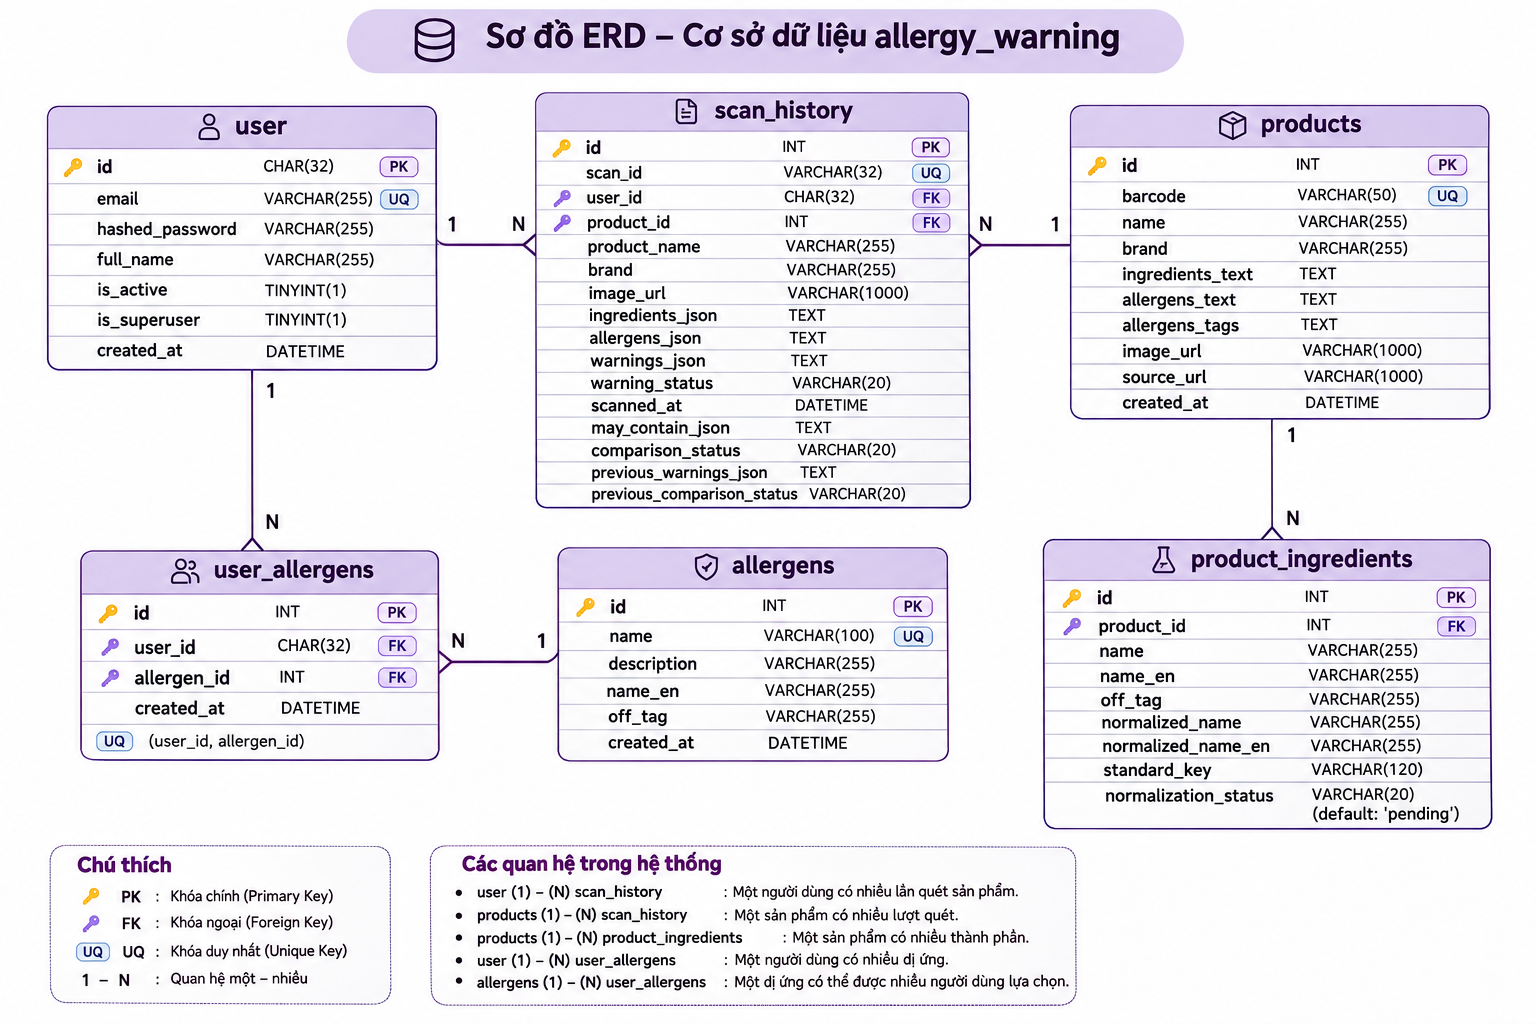
\includegraphics[width=0.98\textwidth,height=0.72\textheight,keepaspectratio]{assets/10_erd_co_so_du_lieu.png}
	\caption{Sơ đồ ERD cập nhật của cơ sở dữ liệu Allergy Warning}
	\label{fig:erd-allergy-warning}
\end{figure}

Sơ đồ cho thấy \texttt{scan\_history} liên kết trực tiếp với \texttt{user} và \texttt{products}; không có quan hệ trực tiếp giữa \texttt{scan\_history} và \texttt{product\_ingredients}. Bảng \texttt{product\_ingredients} chỉ liên kết với \texttt{products} thông qua \texttt{product\_id}. Đây là điểm cần lưu ý để bảo đảm phần mô tả và sơ đồ thống nhất với cấu trúc khóa ngoại thực tế.

\Needspace{9\baselineskip}
\subsection{Nguyên tắc bảo đảm dữ liệu}

\textbf{Tính toàn vẹn:}

Các bảng sử dụng khóa chính để xác định bản ghi. Những mối quan hệ cần thiết được thiết lập bằng khóa ngoại, giúp dữ liệu liên kết đúng đối tượng.

\textbf{Tính duy nhất:}

Email người dùng, tên dị nguyên, mã vạch sản phẩm và mã lần quét có các ràng buộc duy nhất theo cấu trúc cơ sở dữ liệu. Bảng \texttt{user\_allergens} cũng có ràng buộc duy nhất kết hợp giữa người dùng và dị nguyên.

\textbf{Tính nhất quán:}

Thông tin dị nguyên được lưu tập trung trong bảng \texttt{allergens}. Hồ sơ dị ứng tham chiếu đến bảng này, giúp hạn chế việc mỗi người dùng lưu một cách biểu diễn riêng cho cùng một dị nguyên.

\textbf{Tính bảo mật:}

Mật khẩu được lưu dưới dạng giá trị băm trong trường \texttt{hashed\_password}. Việc truy cập lịch sử quét và hồ sơ cá nhân cần được giới hạn theo tài khoản tương ứng.

\textbf{Khả năng mở rộng:}

Cấu trúc bảng cho phép bổ sung sản phẩm, thành phần và nhóm dị nguyên mới. Lịch sử quét cũng có thể lưu nhiều lần phân tích của một người dùng.

% =========================================================
% 3.7 THIẾT KẾ GIAO DIỆN
% =========================================================

\Needspace{12\baselineskip}
\section{Thiết kế giao diện hệ thống}

\Needspace{9\baselineskip}
\subsection{Giao diện đăng nhập}

Giao diện đăng nhập cho phép người dùng nhập email và mật khẩu để truy cập hệ thống. Trang được chia thành khu vực giới thiệu hệ thống và khu vực nhập thông tin tài khoản. Cách bố trí này giúp người dùng dễ nhận biết mục đích của ứng dụng và thao tác đăng nhập.

\begin{figure}[H]
	\centering
	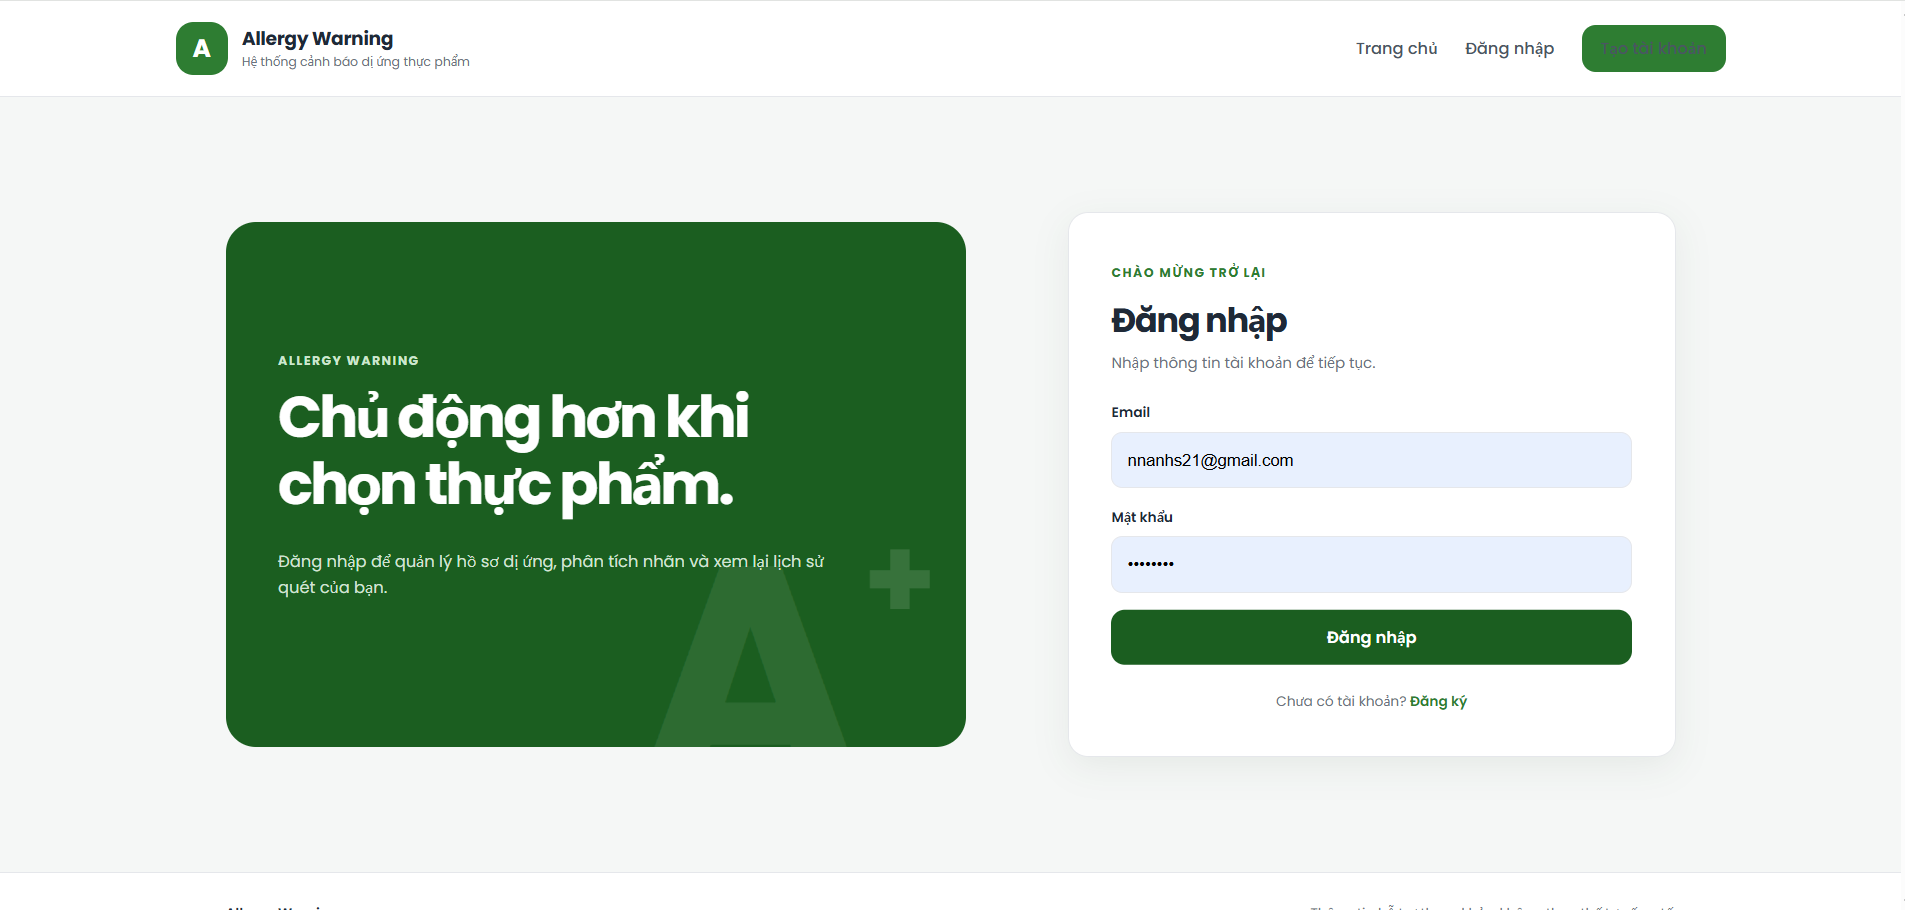
\includegraphics[width=0.90\textwidth,height=0.62\textheight,keepaspectratio]{assets/Login.png}
	\caption{Giao diện đăng nhập hệ thống Allergy Warning}
	\label{fig:giao-dien-dang-nhap}
\end{figure}

Hình minh họa trang đăng nhập, nơi người dùng nhập email và mật khẩu để xác thực trước khi truy cập các chức năng cần tài khoản.


\Needspace{9\baselineskip}
\subsection{Giao diện đăng ký tài khoản}

Giao diện đăng ký cung cấp các trường nhập họ tên, email, mật khẩu và xác nhận mật khẩu. Người dùng nhập thông tin theo yêu cầu của biểu mẫu để tạo tài khoản mới.

\begin{figure}[H]
	\centering
	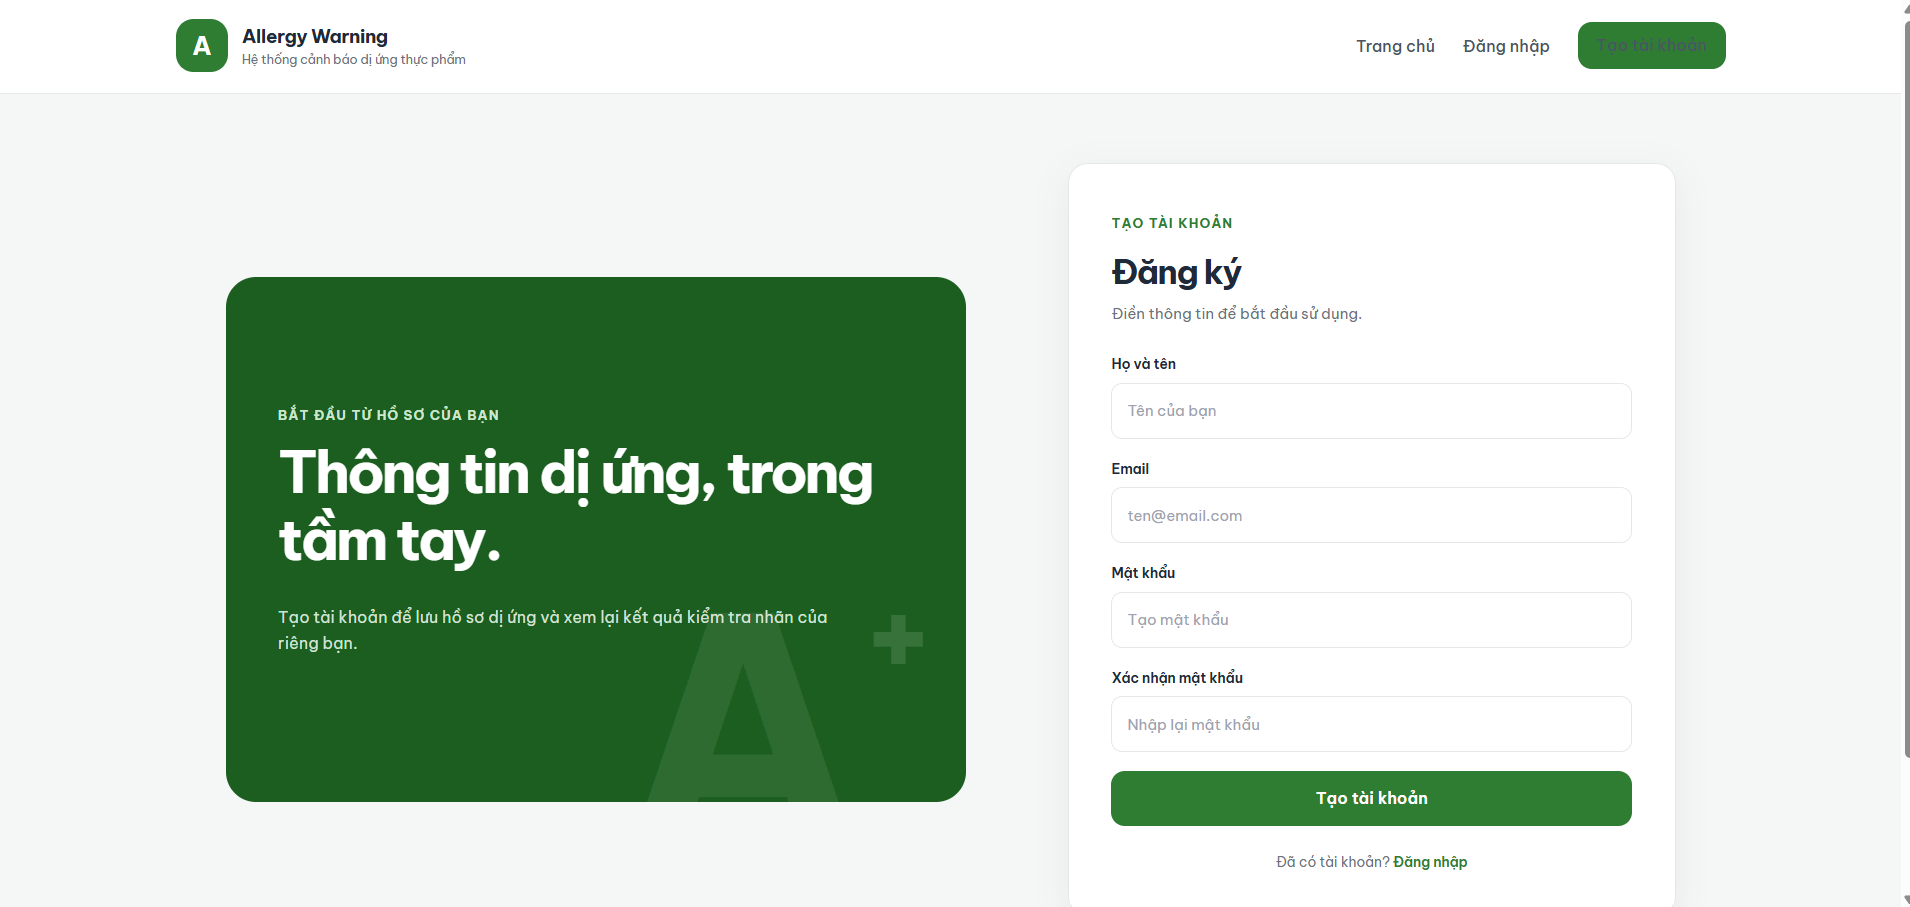
\includegraphics[width=0.90\textwidth,height=0.62\textheight,keepaspectratio]{assets/register.png}
	\caption{Giao diện đăng ký tài khoản}
	\label{fig:giao-dien-dang-ky}
\end{figure}

Hình minh họa biểu mẫu đăng ký, cho phép người dùng nhập thông tin cần thiết để tạo tài khoản mới.


\Needspace{9\baselineskip}
\subsection{Giao diện Dashboard người dùng}

Dashboard là trang tổng quan sau khi người dùng đăng nhập. Giao diện hiển thị lời chào, các lối truy cập nhanh đến chức năng quét nhãn, hồ sơ dị ứng và lịch sử quét. Khu vực hoạt động gần đây giúp người dùng theo dõi các sản phẩm đã phân tích.

\begin{figure}[H]
	\centering
	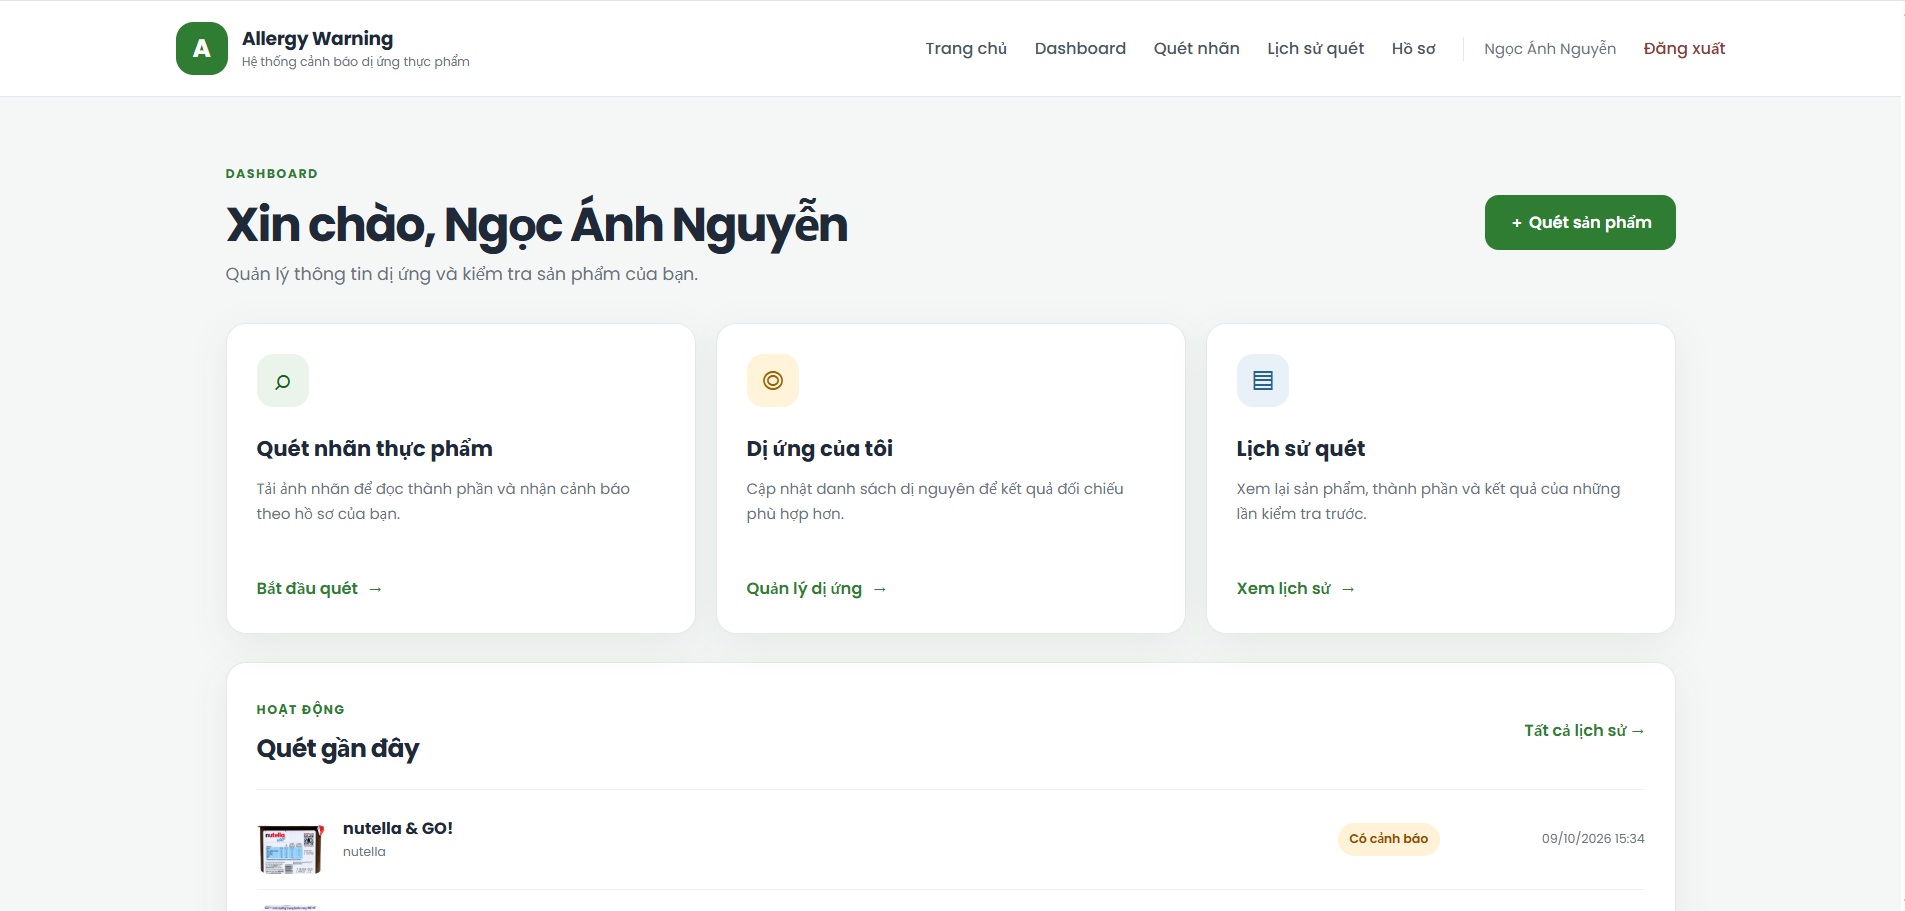
\includegraphics[width=0.95\textwidth,height=0.62\textheight,keepaspectratio]{assets/Dashboard.png}
	\caption{Giao diện Dashboard dành cho người dùng}
	\label{fig:giao-dien-dashboard}
\end{figure}

Hình minh họa trang tổng quan sau đăng nhập, cung cấp lối truy cập đến các chức năng chính và thông tin hoạt động của người dùng.


\Needspace{9\baselineskip}
\subsection{Giao diện hồ sơ cá nhân}

Giao diện hồ sơ cá nhân cung cấp thông tin tài khoản và những thông tin chất gây dị ứng  liên quan đến người dùng.

\begin{figure}[H]
	\centering
	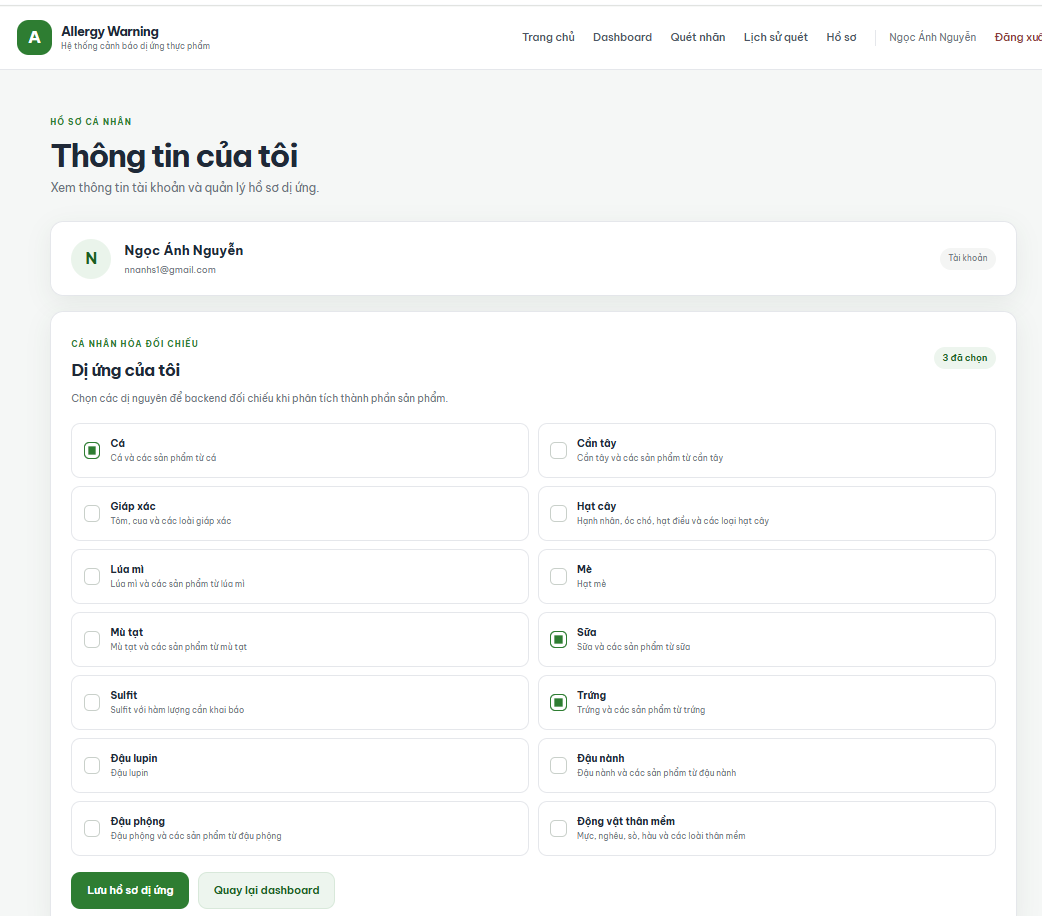
\includegraphics[width=0.90\textwidth,height=0.62\textheight,keepaspectratio]{assets/profile.png}
	\caption{Giao diện hồ sơ cá nhân - phần thông tin dị ứng của  tài khoản}
	\label{fig:giao-dien-ho-so-1}
\end{figure}

Hình thể hiện khu vực thông tin tài khoản trong trang hồ sơ cá nhân, giúp người dùng có thể kiểm tra, theo dõi hoặc cập nhật lại thông tin của bản thân.

\Needspace{9\baselineskip}
\subsection{Giao diện quét nhãn thực phẩm}

Giao diện quét nhãn cho phép người dùng tải ảnh từ thiết bị. Sau khi chọn ảnh, hệ thống hiển thị ảnh hoặc tên tệp và nút bắt đầu phân tích. Phần hướng dẫn trên giao diện cung cấp thông tin về định dạng ảnh được hỗ trợ.

\begin{figure}[H]
	\centering
	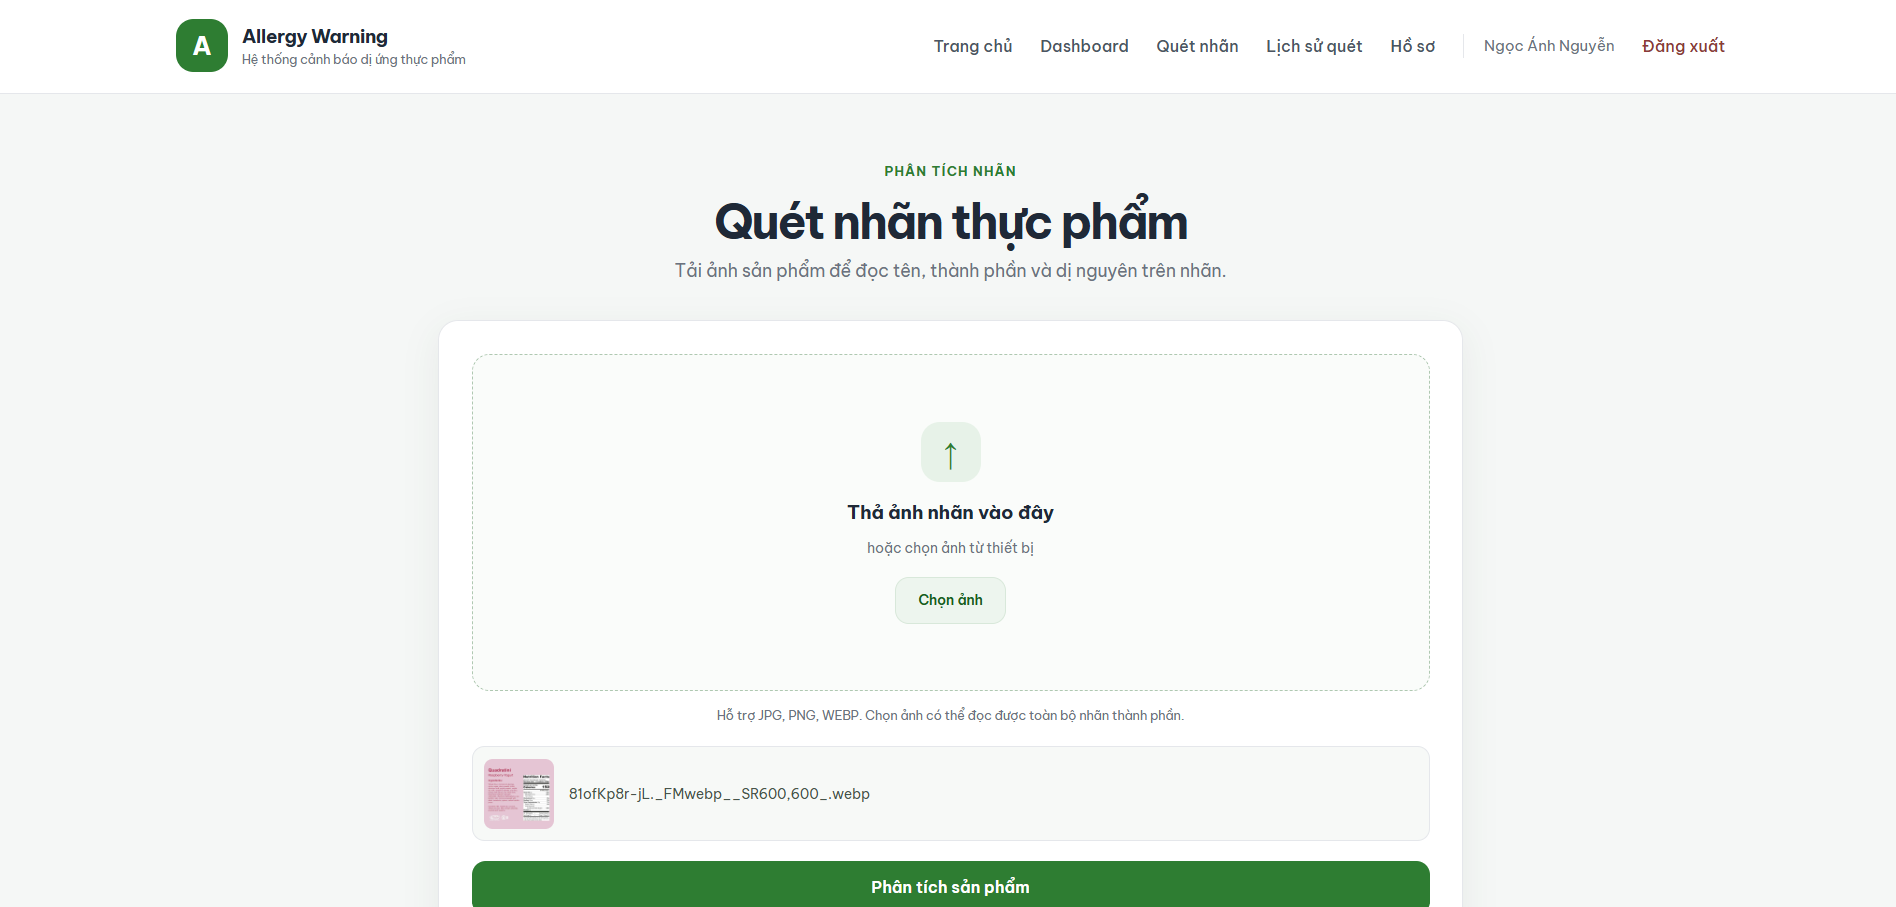
\includegraphics[width=0.90\textwidth,height=0.62\textheight,keepaspectratio]{assets/scan.png}
	\caption{Giao diện tải ảnh nhãn thực phẩm}
	\label{fig:giao-dien-quet-nhan}
\end{figure}

Hình minh họa giao diện chọn và tải ảnh nhãn thực phẩm trước khi gửi yêu cầu phân tích.


\Needspace{9\baselineskip}
\subsection{Giao diện lịch sử quét}

Giao diện lịch sử quét giúp người dùng xem lại các sản phẩm đã được phân tích. Mỗi bản ghi có thể hiển thị tên sản phẩm, hình ảnh, trạng thái cảnh báo và thời gian thực hiện.

\begin{figure}[H]
	\centering
	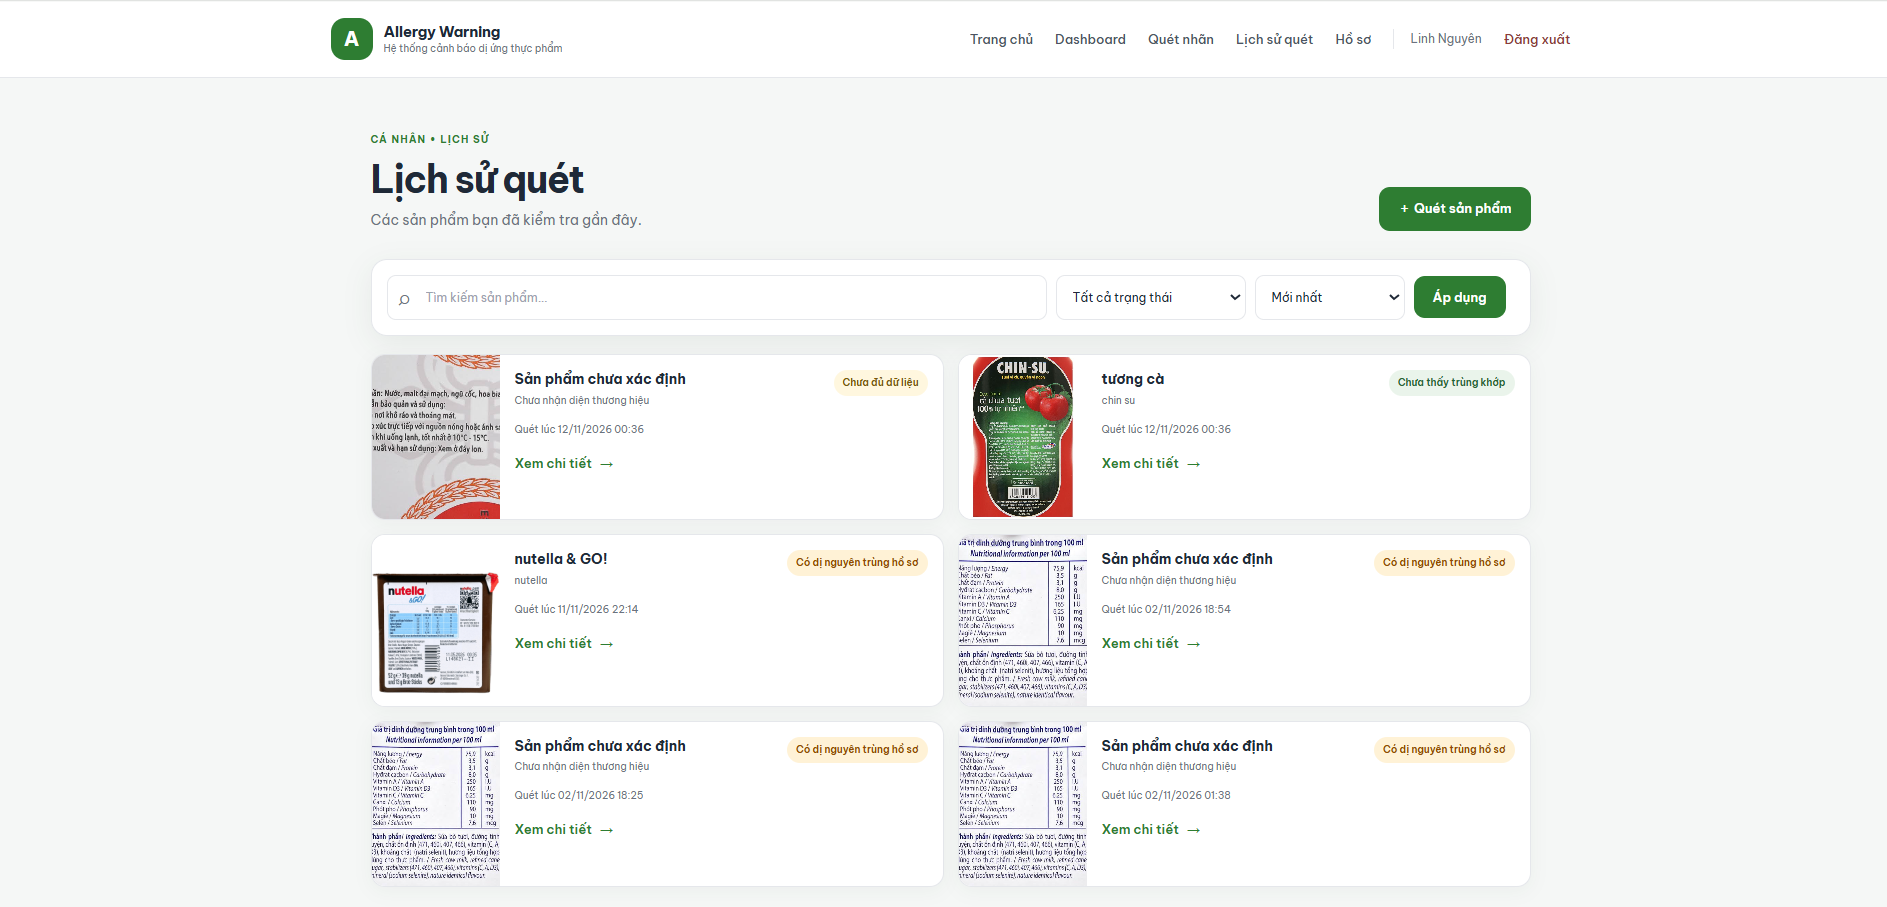
\includegraphics[width=0.95\textwidth,height=0.62\textheight,keepaspectratio]{assets/scan_history.png}
	\caption{Giao diện danh sách lịch sử quét}
	\label{fig:giao-dien-lich-su}
\end{figure}

Hình minh họa danh sách các lần quét đã lưu, giúp người dùng tra cứu sản phẩm, thời điểm và trạng thái cảnh báo.


\Needspace{9\baselineskip}
\subsection{Giao diện chi tiết lịch sử quét}

Các ảnh chi tiết lịch sử quét minh họa những phần thông tin khác nhau của một bản ghi, bao gồm thông tin sản phẩm, nội dung phân tích và cảnh báo dị nguyên. Việc tách thành nhiều ảnh giúp thể hiện đầy đủ nội dung của trang chi tiết.

\begin{figure}[H]
	\centering
	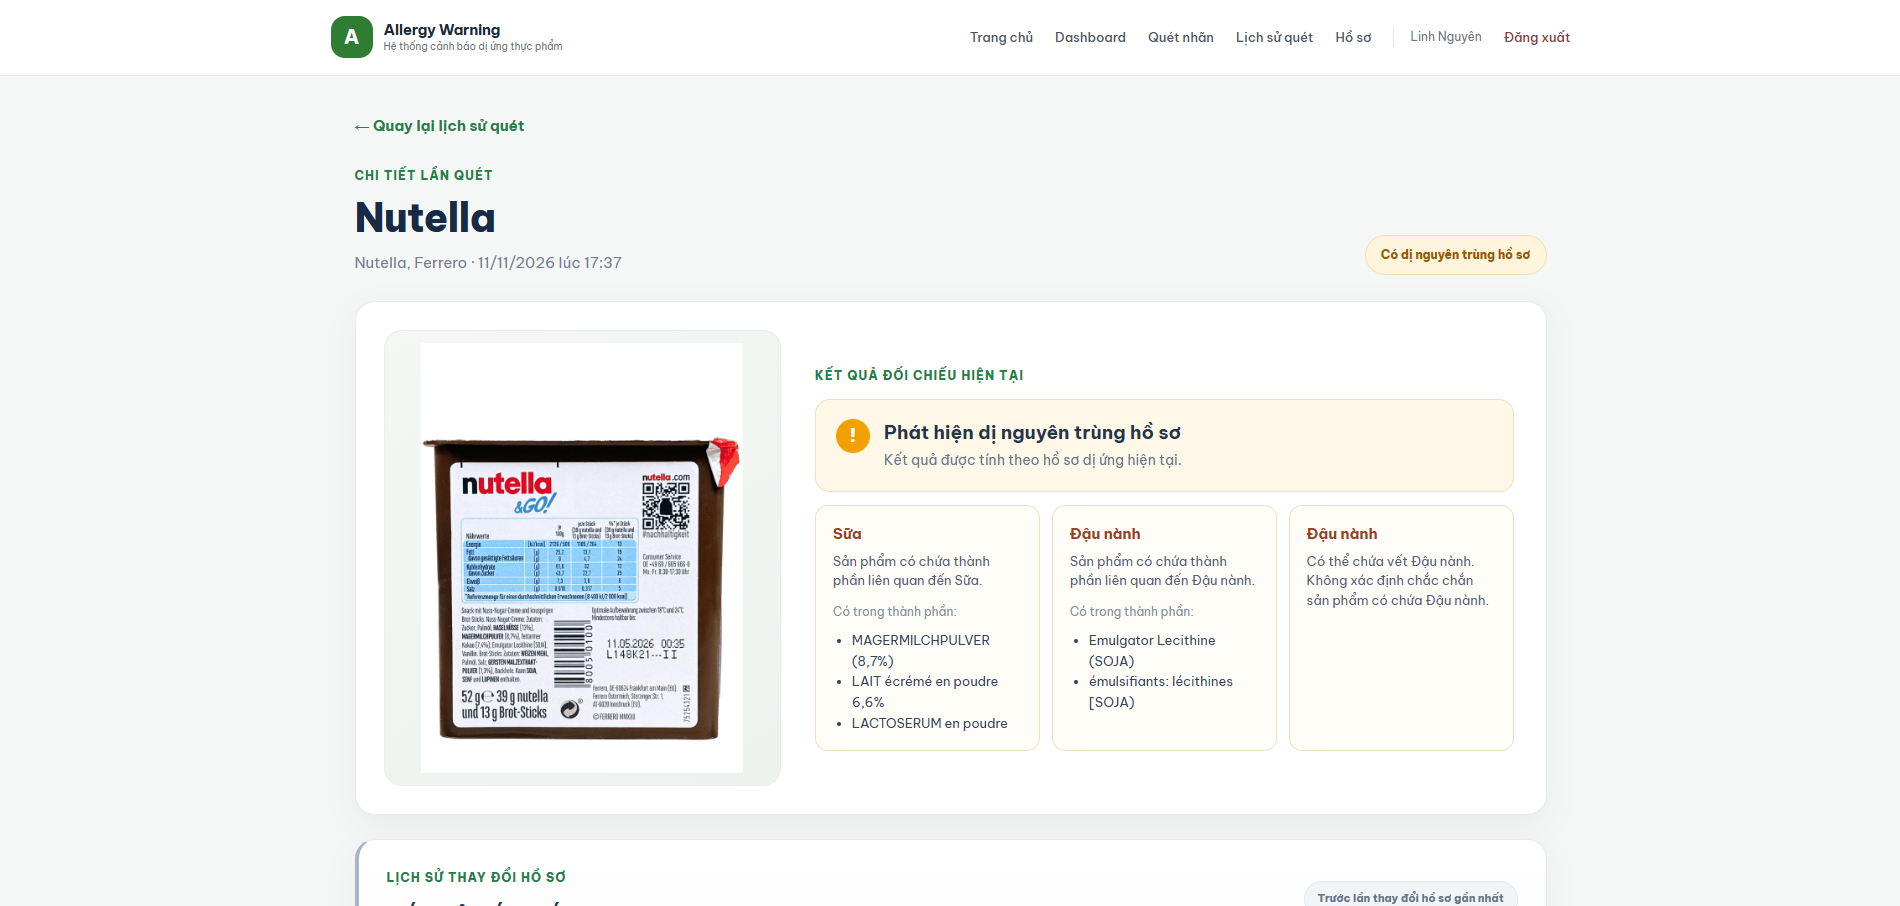
\includegraphics[width=0.90\textwidth,height=0.62\textheight,keepaspectratio]{assets/scan_history_product_detail1.png}
	\caption{Chi tiết lịch sử quét - thông tin sản phẩm}
	\label{fig:lich-su-chi-tiet-1}
\end{figure}

Hình thể hiện phần thông tin sản phẩm của một bản ghi lịch sử quét, giúp người dùng nhận biết sản phẩm đã được phân tích.


\begin{figure}[H]
	\centering
	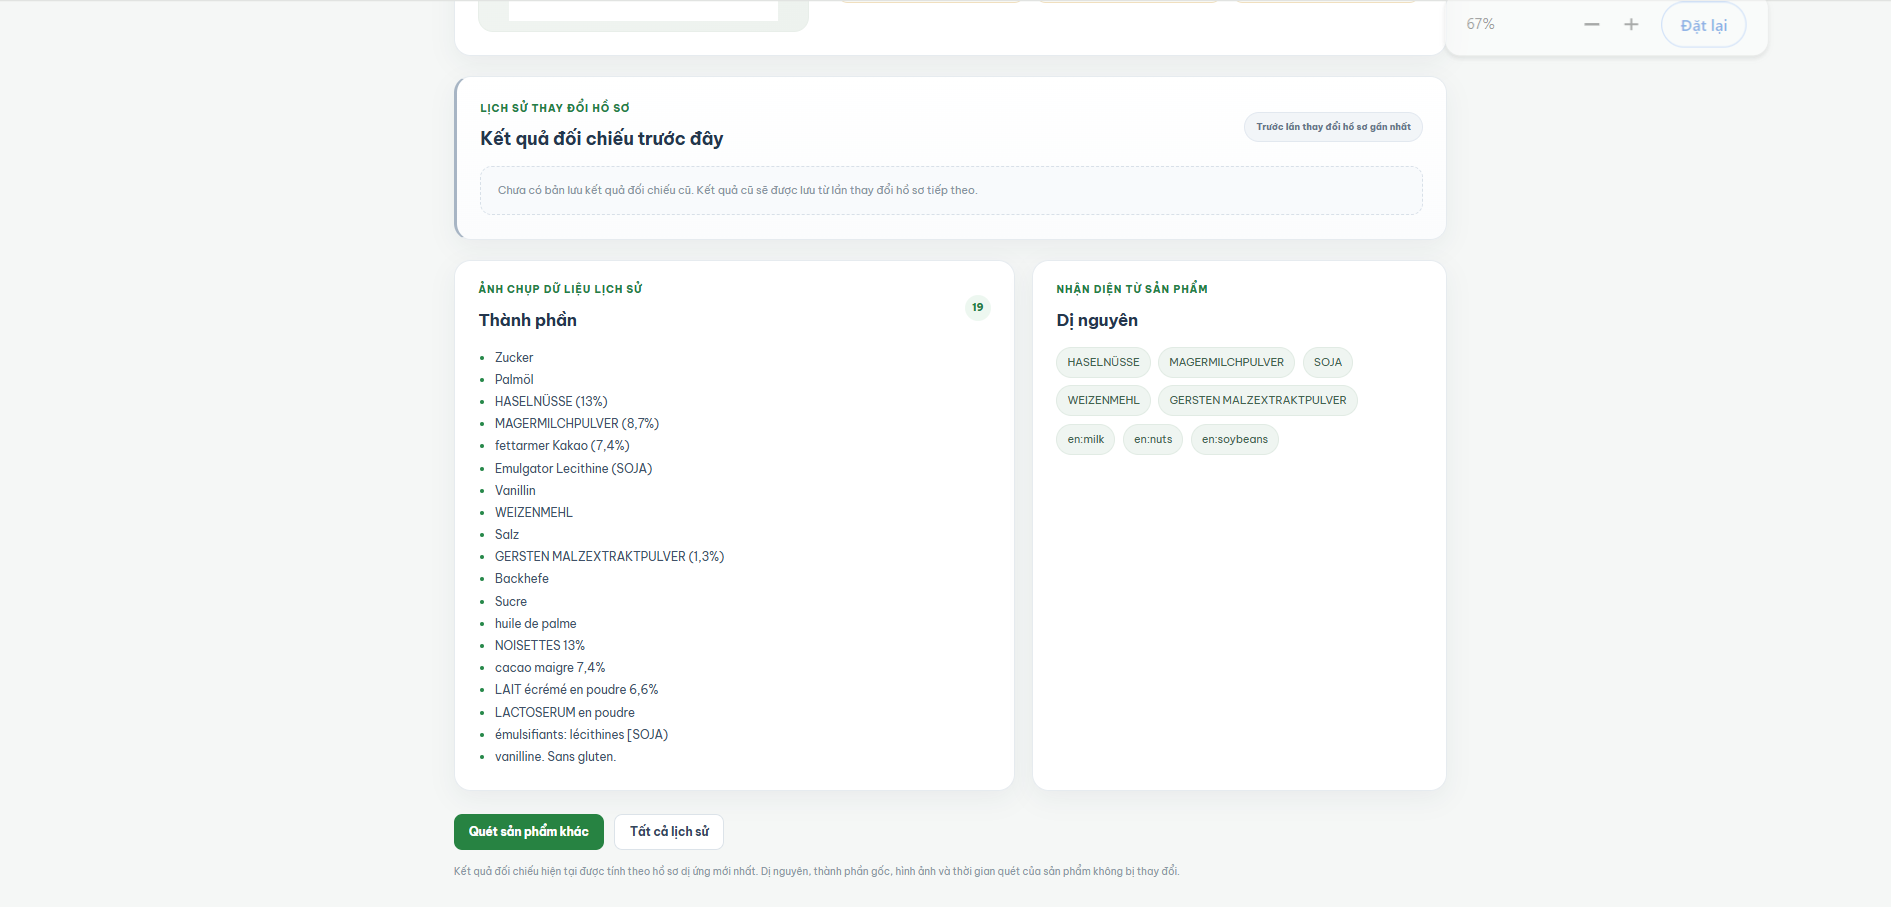
\includegraphics[width=0.90\textwidth,height=0.62\textheight,keepaspectratio]{assets/scan_history_product_detail2.png}
	\caption{Chi tiết lịch sử quét - thông tin phân tích}
	\label{fig:lich-su-chi-tiet-2}
\end{figure}

Hình thể hiện phần thông tin phân tích của bản ghi, bổ sung chi tiết thành phần và kết quả cảnh báo tương ứng.




\Needspace{9\baselineskip}
\subsection{Giao diện kết quả phân tích}

Giao diện kết quả phân tích hiển thị thông tin thu được sau khi hệ thống xử lý ảnh nhãn thực phẩm. Ba hình ảnh liên tiếp minh họa ba phần của cùng một trang kết quả, không phải ba giao diện độc lập.

Phần đầu giao diện hiển thị tên sản phẩm, thương hiệu, hình ảnh nhãn thực phẩm và trạng thái cảnh báo tổng quan. Phần tiếp theo trình bày danh sách thành phần được nhận diện và các dị nguyên được phát hiện. Phần cuối trình bày chi tiết cảnh báo dị nguyên, bao gồm các dị nguyên có bằng chứng trong danh sách thành phần và những thông tin cảnh báo có thể chứa vết dị nguyên trên nhãn.

\begin{figure}[H]
	\centering
	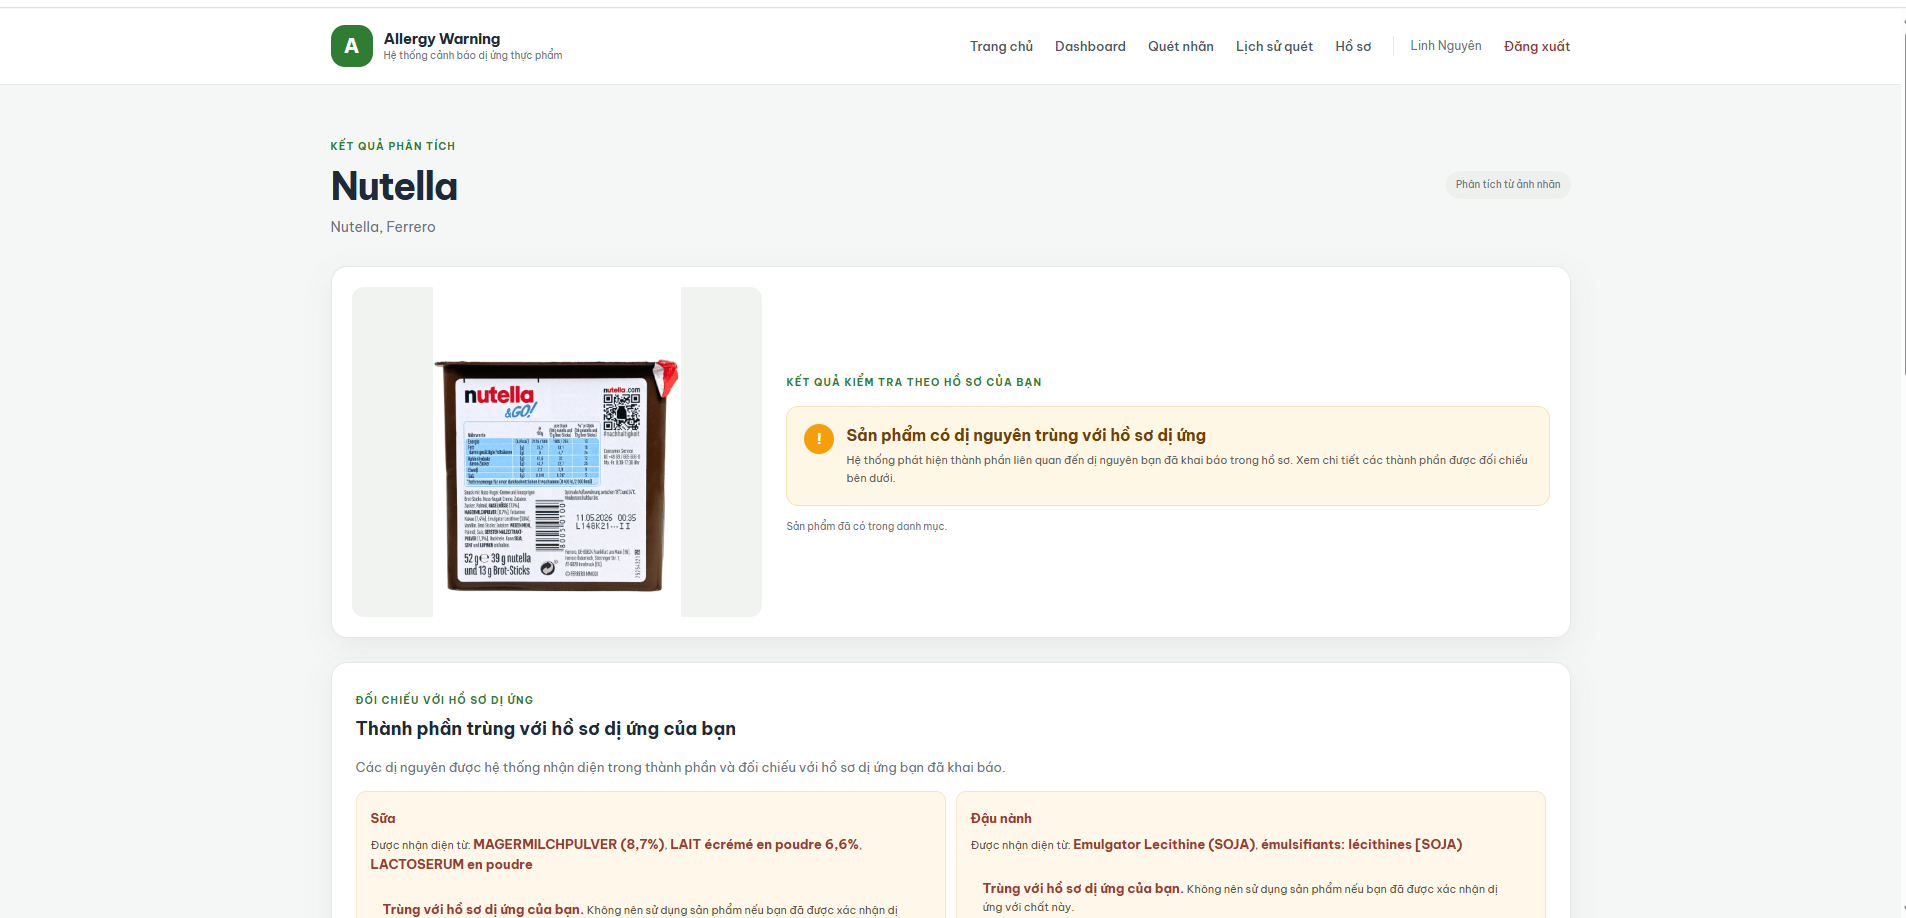
\includegraphics[width=0.90\textwidth,height=0.62\textheight,keepaspectratio]{assets/result1.png}
	\caption{Phần đầu giao diện kết quả phân tích sản phẩm}
	\label{fig:giao-dien-ket-qua-1}
\end{figure}

Hình minh họa phần đầu trang kết quả, gồm thông tin nhận diện sản phẩm và trạng thái cảnh báo tổng quan.


\begin{figure}[H]
	\centering
	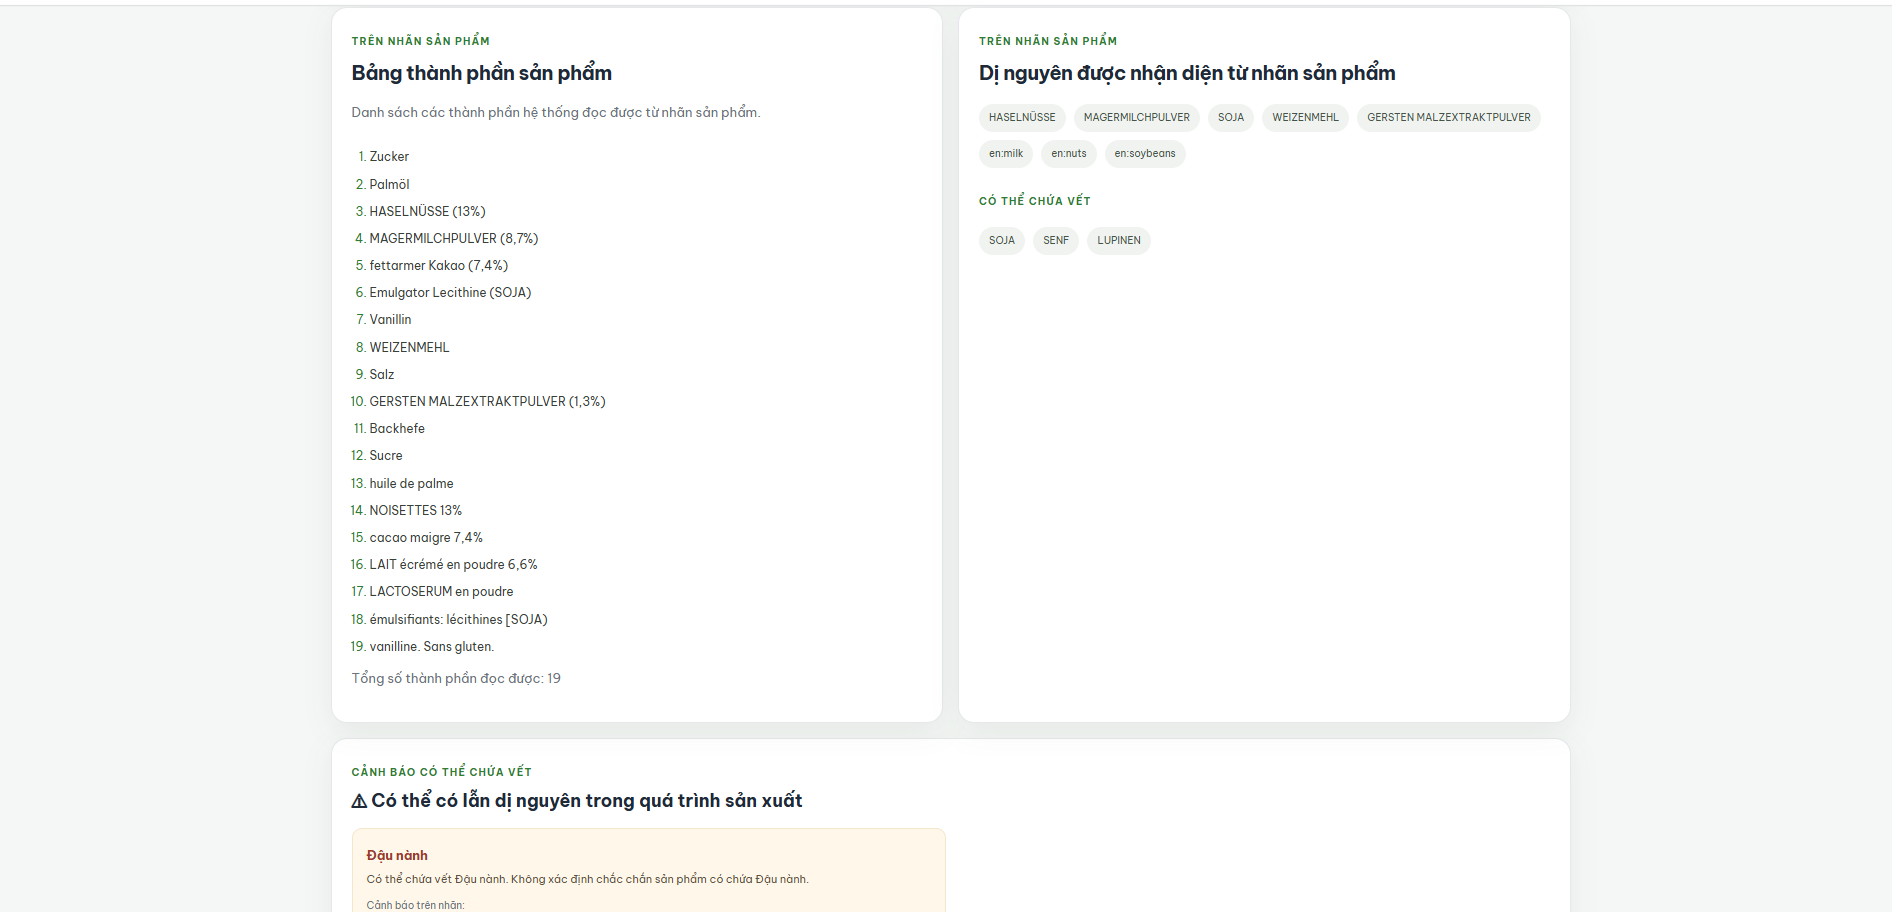
\includegraphics[width=0.90\textwidth,height=0.62\textheight,keepaspectratio]{assets/result2.png}
	\caption{Phần hiển thị chi tiết thành phần và dị nguyên}
	\label{fig:giao-dien-ket-qua-2}
\end{figure}

Hình minh họa khu vực trình bày thành phần được nhận diện và những dị nguyên có liên quan trong kết quả phân tích.


\begin{figure}[H]
	\centering
	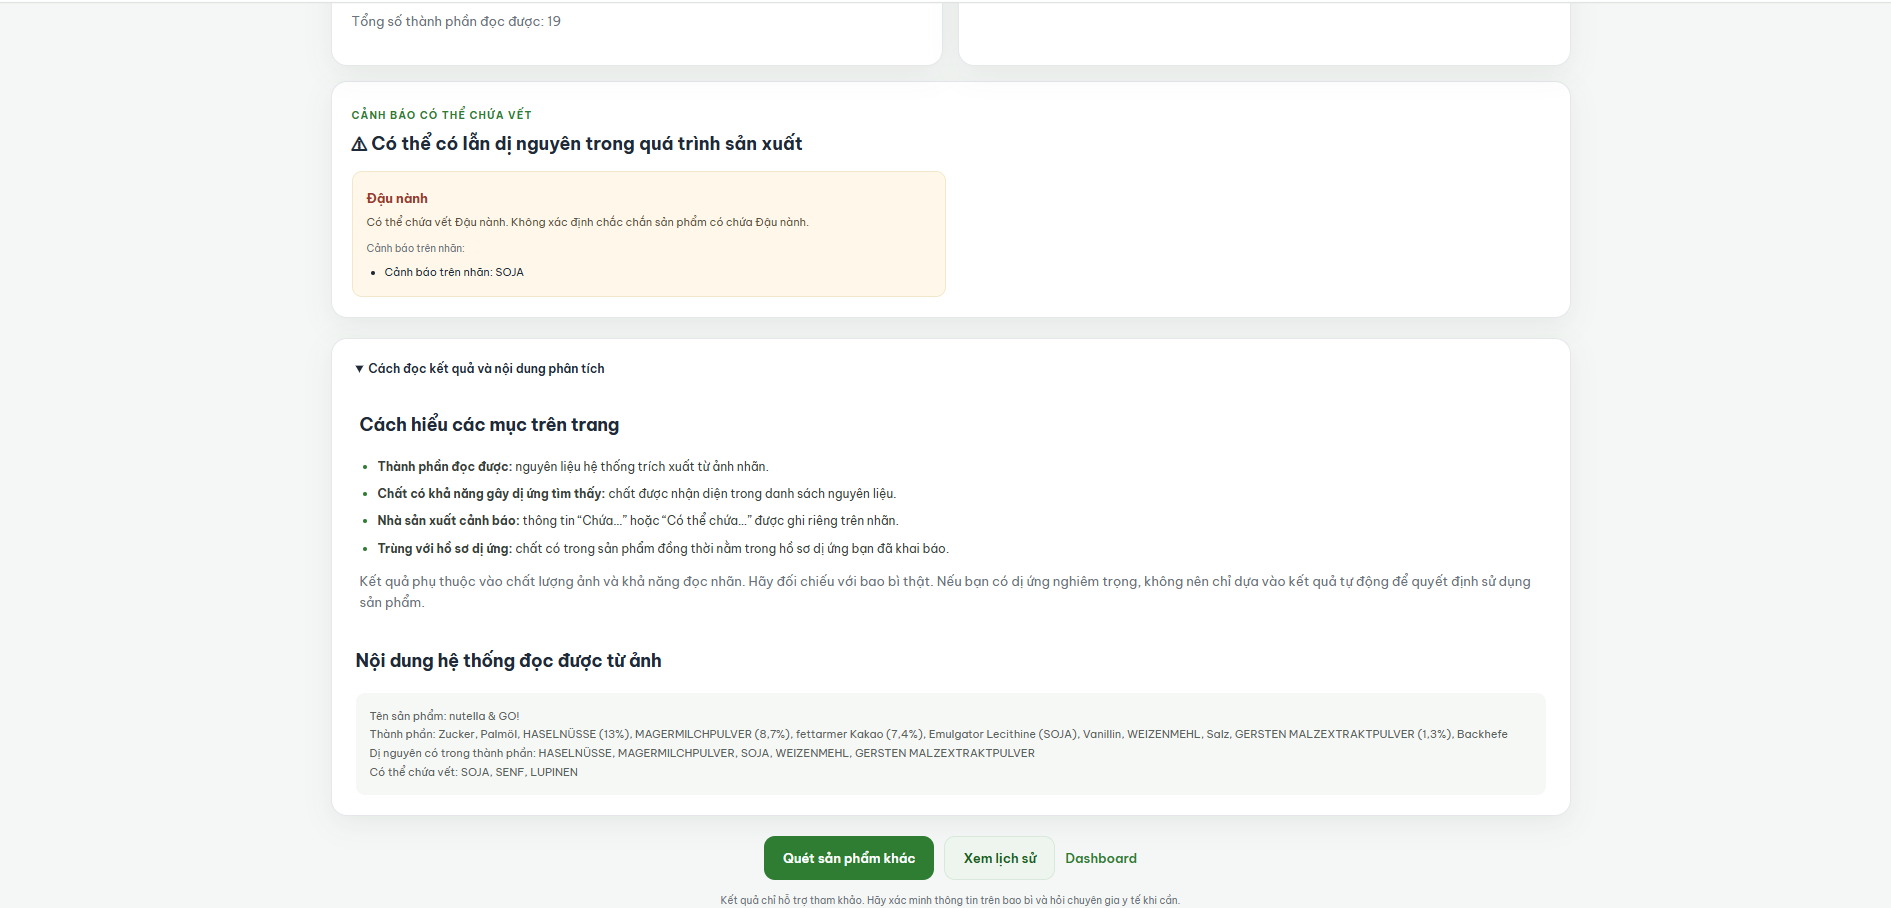
\includegraphics[width=0.90\textwidth,height=0.62\textheight,keepaspectratio]{assets/result3.png}
	\caption{Phần hiển thị chi tiết cảnh báo dị nguyên}
	\label{fig:giao-dien-ket-qua-3}
\end{figure}

Hình minh họa phần chi tiết cảnh báo, trong đó phân biệt dị nguyên có bằng chứng trong thành phần và cảnh báo có thể chứa vết.


Ba hình trên minh họa các phần khác nhau của cùng một giao diện kết quả phân tích. Việc trình bày liên tiếp giúp thể hiện đầy đủ thông tin sản phẩm, thành phần được nhận diện và các cảnh báo liên quan trong quá trình hệ thống hỗ trợ người dùng kiểm tra nhãn thực phẩm.

% =========================================================
% 3.8 GIAO DIỆN QUẢN TRỊ
% =========================================================

\Needspace{12\baselineskip}
\section{Thiết kế giao diện quản trị}

Khu vực quản trị được thiết kế dành cho tài khoản có quyền quản trị. Các màn hình minh họa thể hiện trang tổng quan, khu vực dữ liệu và chức năng xem thông tin sản phẩm. Giao diện sử dụng phong cách trình bày thống nhất với hệ thống, giúp quản trị viên thuận tiện theo dõi và thao tác.

\Needspace{9\baselineskip}
\subsection{Dashboard quản trị}

Dashboard quản trị cung cấp cái nhìn tổng quan về dữ liệu và hoạt động của hệ thống. Các thông tin được bố trí thành những khu vực riêng biệt để quản trị viên dễ theo dõi.

\begin{figure}[H]
	\centering
	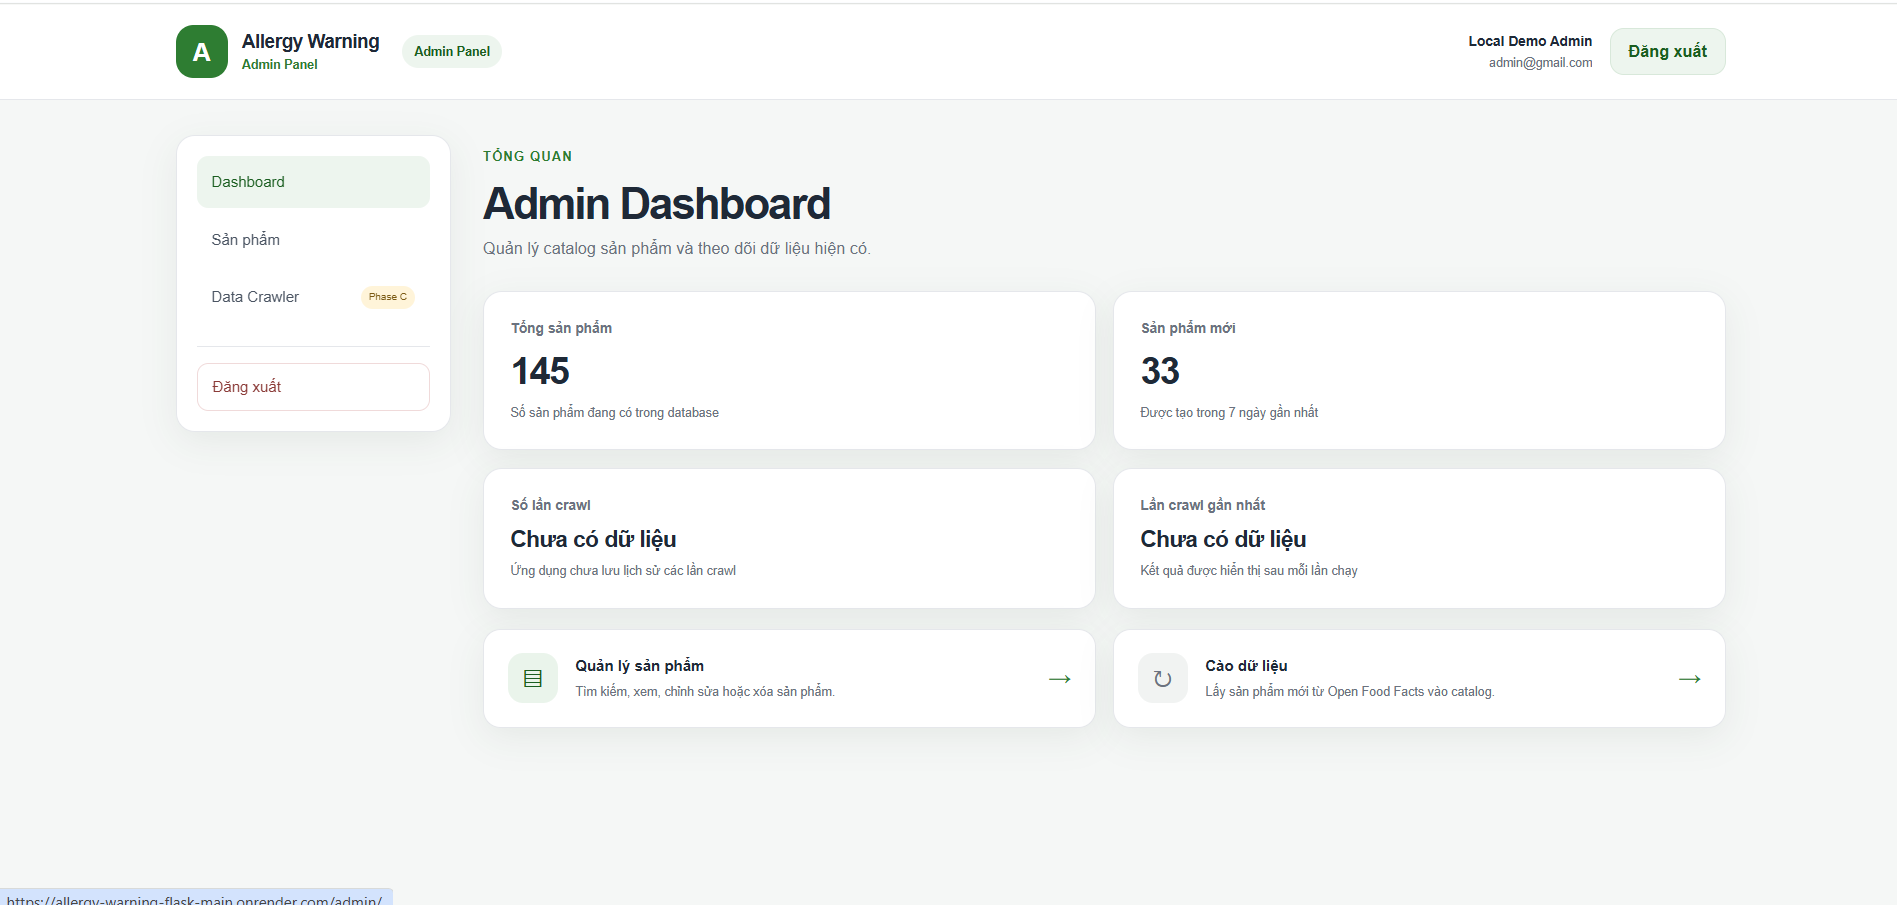
\includegraphics[width=0.95\textwidth,height=0.62\textheight,keepaspectratio]{assets/admin_dashboard.png}
	\caption{Giao diện Dashboard quản trị}
	\label{fig:admin-dashboard}
\end{figure}

Hình minh họa Dashboard quản trị, nơi hiển thị thông tin tổng quan phục vụ việc theo dõi hoạt động và dữ liệu hệ thống.


\Needspace{9\baselineskip}
\subsection{Giao diện lấy thông tin sản phẩm}

Giao diện này cho phép quản trị viên lấy thông tin sản phẩm để lưu vào hệ thống.

\begin{figure}[H]
	\centering
	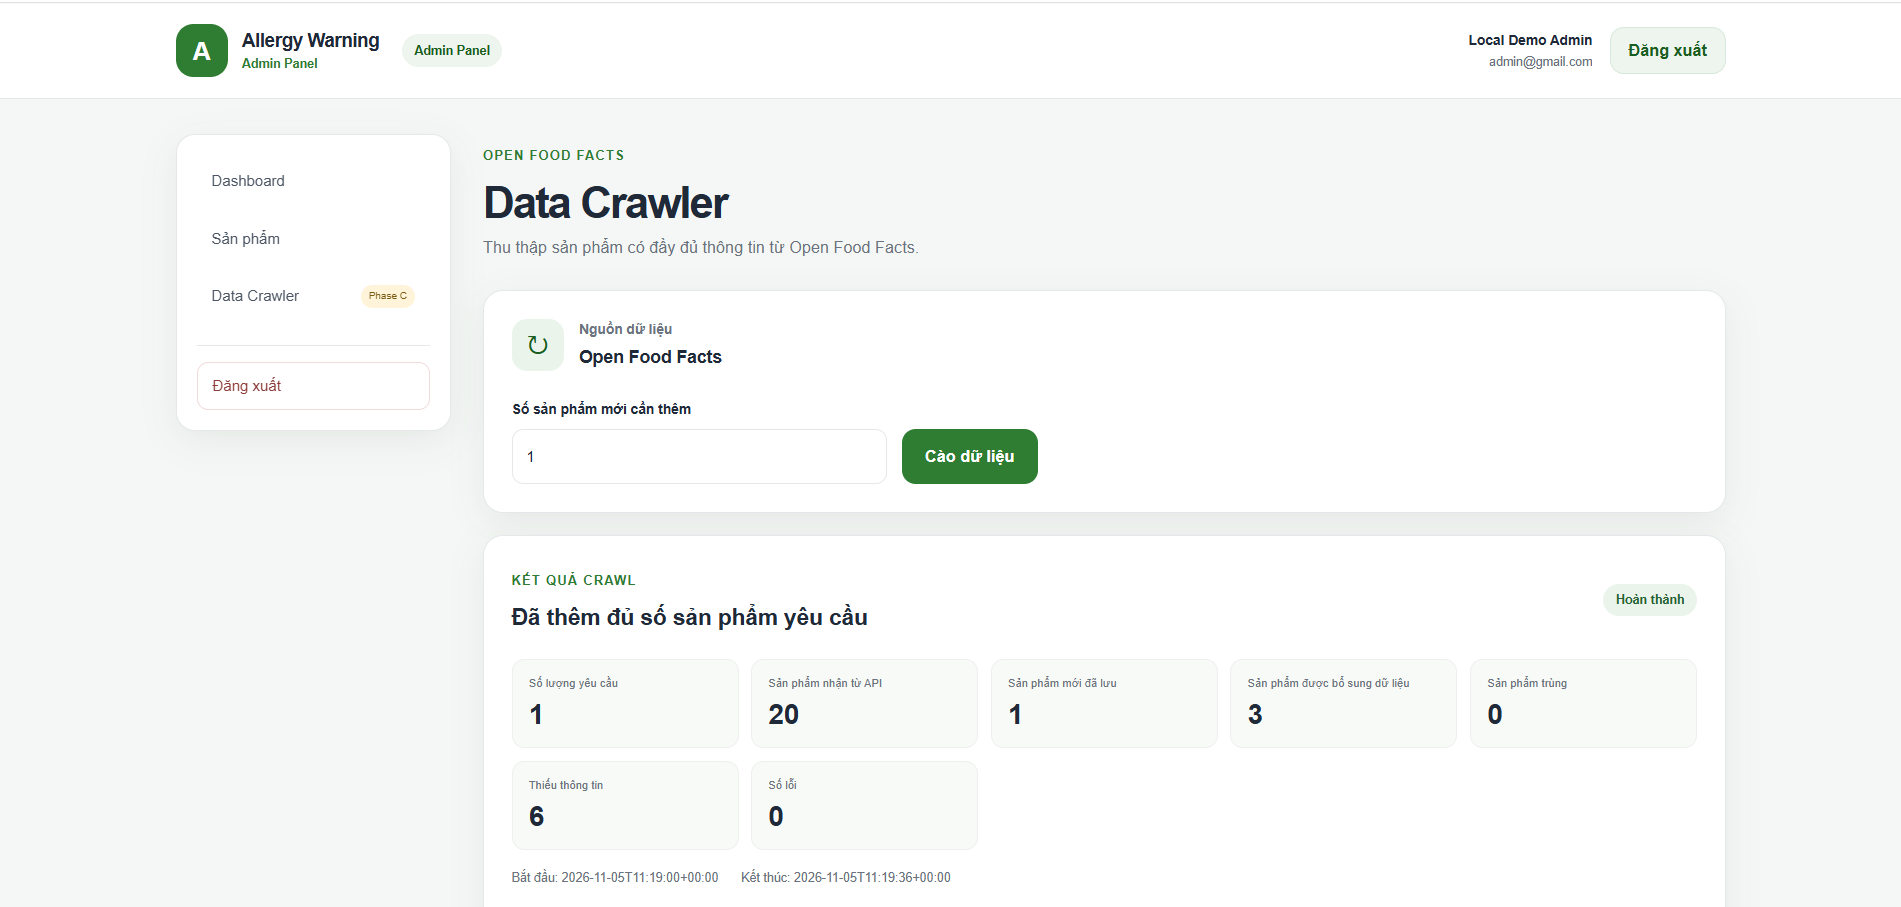
\includegraphics[width=0.95\textwidth,height=0.62\textheight,keepaspectratio]{assets/admin_data1.png}
	\caption{Giao diện thu thập dữ liệu - màn hình thứ nhất}
	\label{fig:admin-data-1}
\end{figure}

Hình minh họa màn hình đầu tiên của chức năng thu thập dữ liệu sản phẩm trong khu vực quản trị.


\begin{figure}[H]
	\centering
	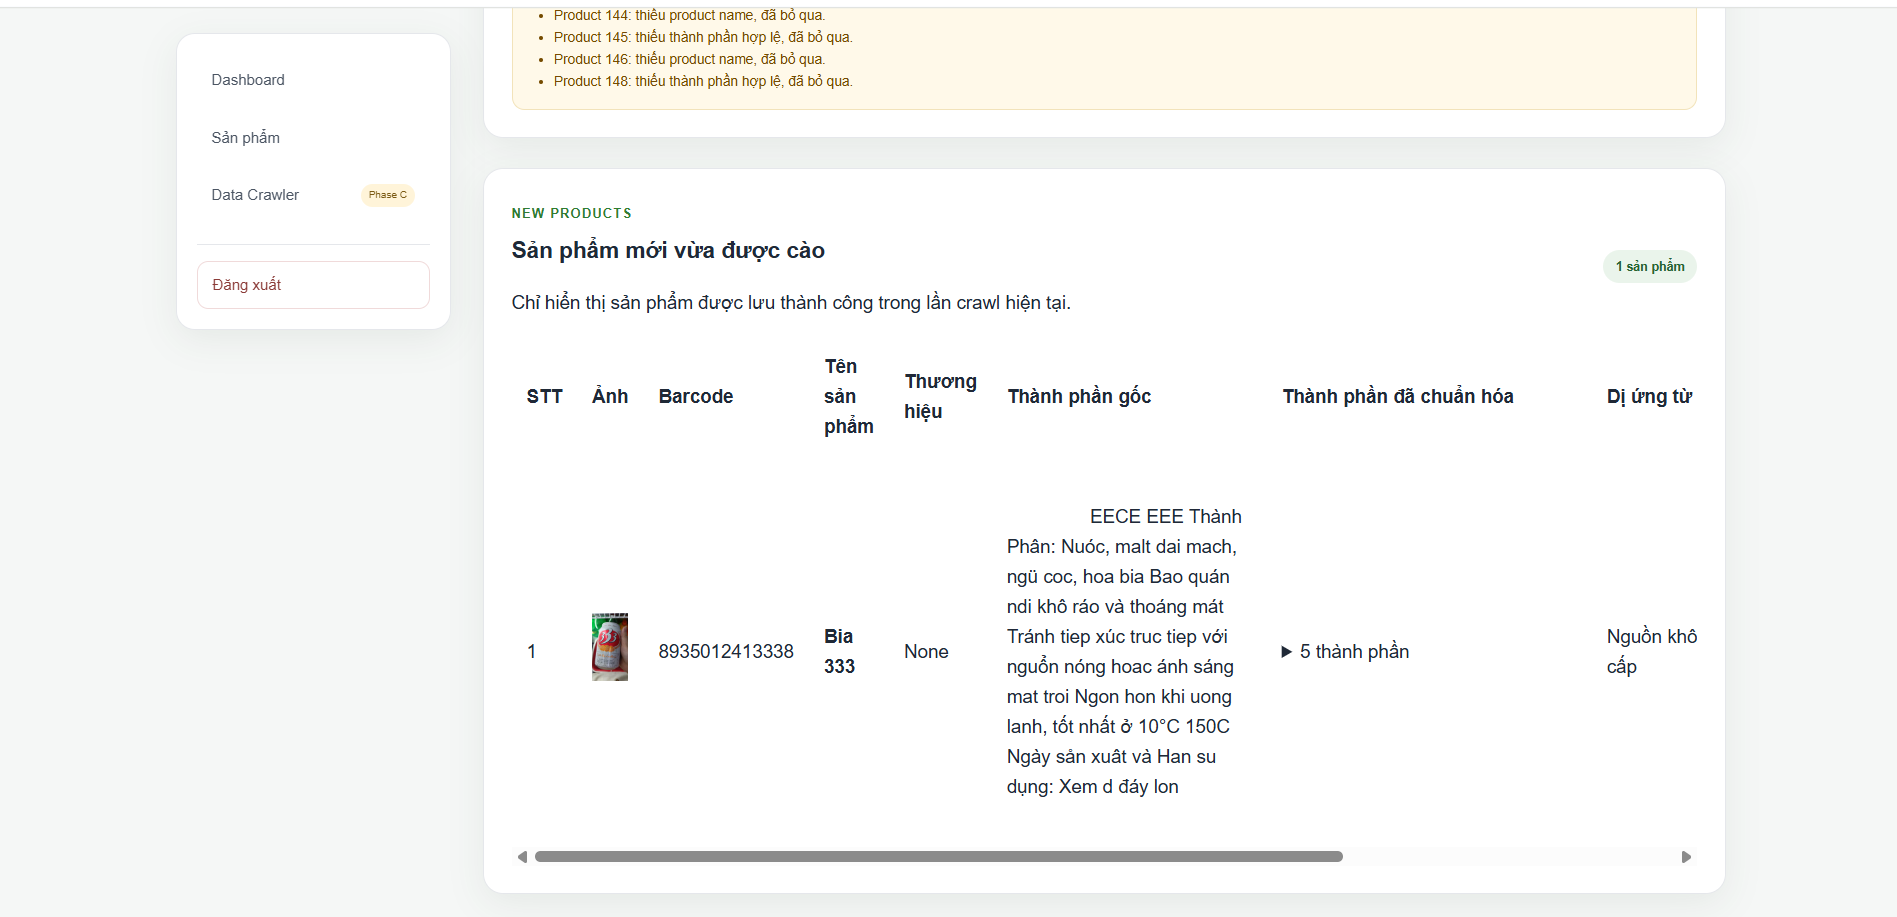
\includegraphics[width=0.95\textwidth,height=0.62\textheight,keepaspectratio]{assets/admin_data2.png}
	\caption{Giao diện thu thập dữ liệu - màn hình thứ hai}
	\label{fig:admin-data-2}
\end{figure}

Hình minh họa màn hình tiếp theo của chức năng thu thập dữ liệu, bổ sung các thao tác và thông tin phục vụ quá trình đưa dữ liệu vào hệ thống.


\Needspace{9\baselineskip}
\subsection{Giao diện quản lý sản phẩm}

Giao diện quản lý sản phẩm thể hiện khu vực quản trị danh sách sản phẩm. Quản trị viên có thể theo dõi các thông tin sản phẩm được hiển thị trong bảng dữ liệu và truy cập trang chi tiết để xem thêm thông tin tương ứng.

\begin{figure}[H]
	\centering
	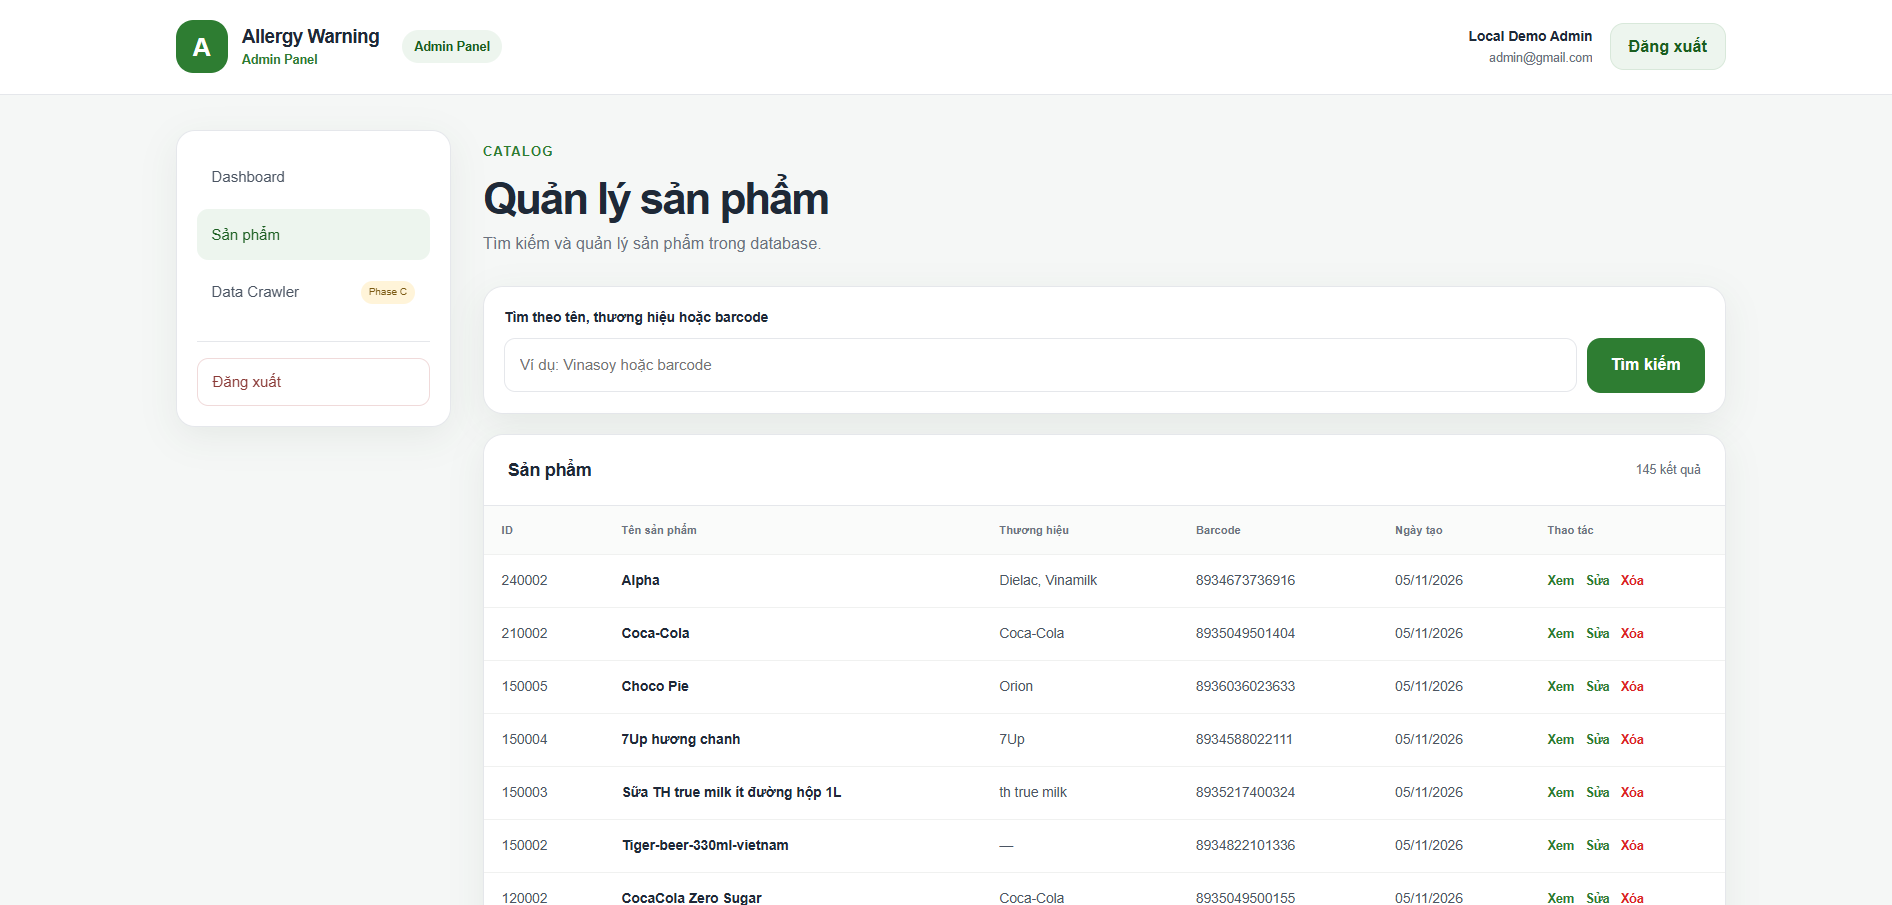
\includegraphics[width=0.95\textwidth,height=0.62\textheight,keepaspectratio]{assets/admin_product.png}
	\caption{Giao diện danh sách sản phẩm trong khu vực quản trị}
	\label{fig:admin-product}
\end{figure}

Hình minh họa danh sách sản phẩm được lưu trong hệ thống, hỗ trợ quản trị viên tra cứu và theo dõi dữ liệu.


\begin{figure}[H]
	\centering
	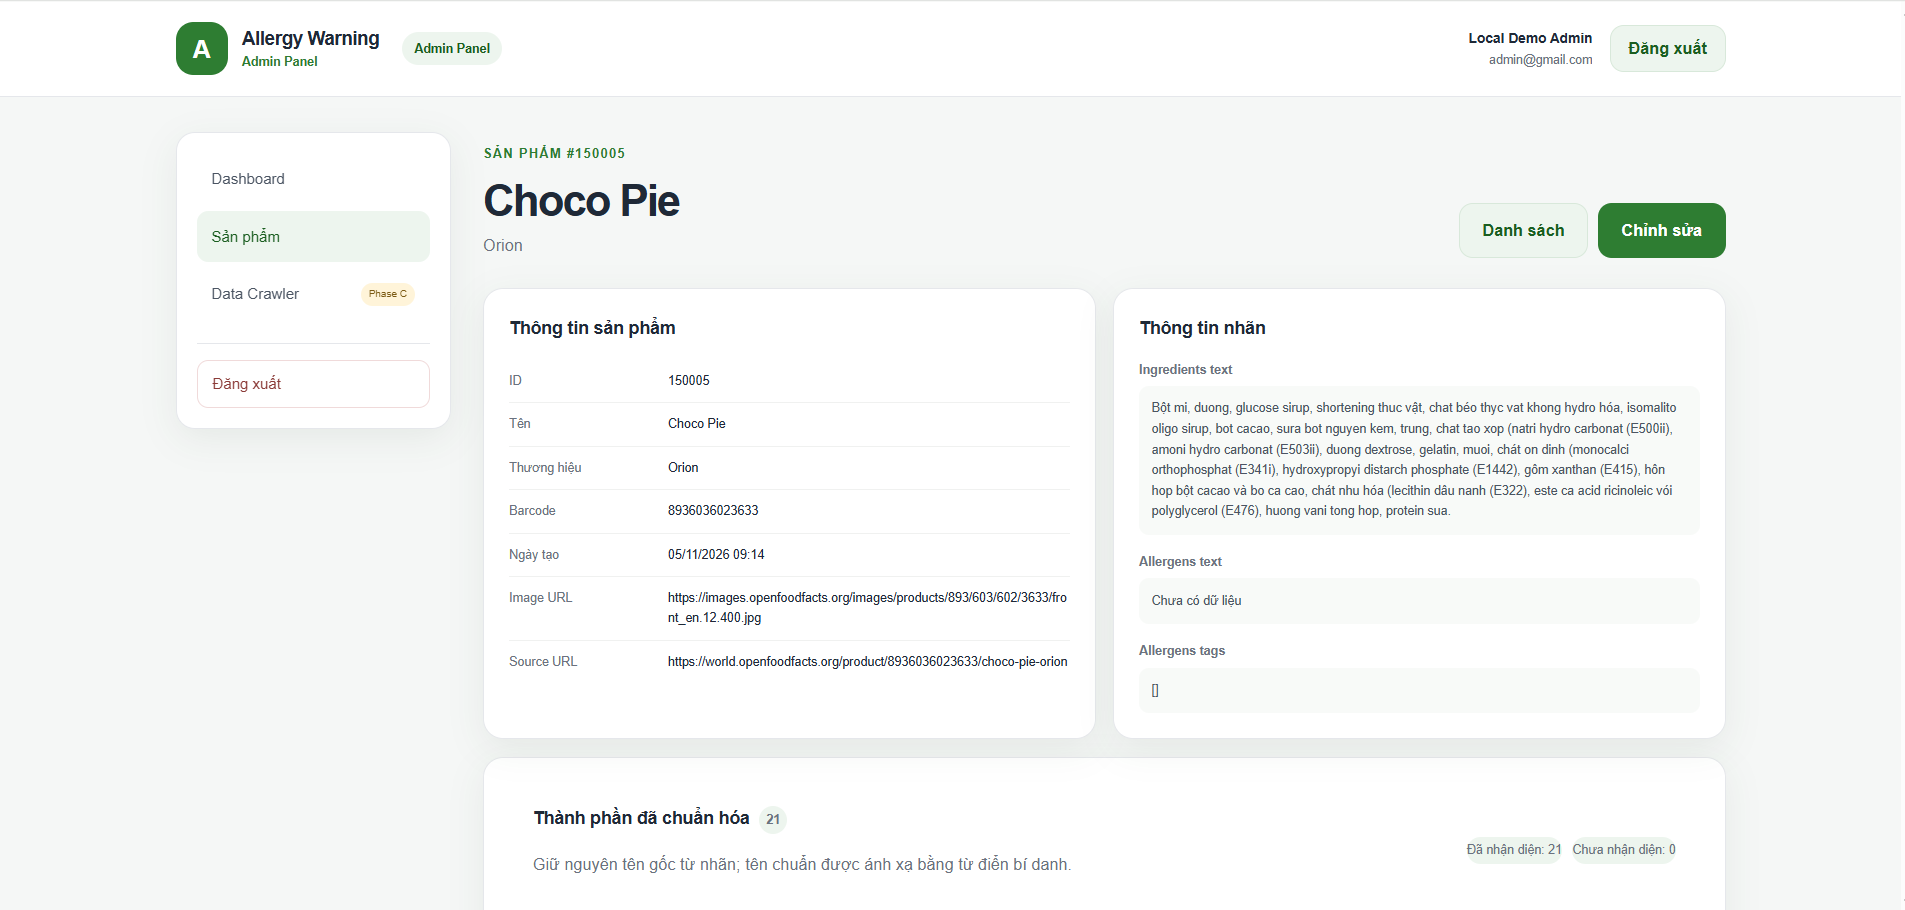
\includegraphics[width=0.95\textwidth,height=0.62\textheight,keepaspectratio]{assets/admin_productdetail.png}
	\caption{Giao diện chi tiết sản phẩm trong khu vực quản trị}
	\label{fig:admin-product-detail}
\end{figure}

Hình minh họa trang chi tiết của một sản phẩm, cung cấp thông tin cụ thể hơn so với bảng danh sách.


% =========================================================
% 3.9 KẾT LUẬN CHƯƠNG
% =========================================================

\Needspace{12\baselineskip}
\section{Kết luận chương}

Chương 3 đã trình bày quá trình phân tích bài toán, xác định đối tượng sử dụng, các yêu cầu chức năng và phi chức năng của hệ thống Allergy Warning. Từ những yêu cầu đó, chương đã mô tả kiến trúc tổng thể, vai trò của Flask, Gemini API, Cloudinary và cơ sở dữ liệu, đồng thời trình bày quy trình quét nhãn, phân tích và phân loại cảnh báo dị nguyên.

Bên cạnh đó, chương đã trình bày cấu trúc cơ sở dữ liệu \texttt{food\_allergen\_system} với sáu bảng chính gồm \texttt{user}, \texttt{allergens}, \texttt{products}, \texttt{product\_ingredients}, \texttt{user\_allergens} và \texttt{scan\_history}. Các bảng được mô tả theo trường dữ liệu và mối quan hệ nhằm làm rõ cách tổ chức thông tin phục vụ hoạt động của hệ thống.

Chương cũng trình bày các sơ đồ Use Case, kiến trúc, quy trình, ERD và các giao diện người dùng, quản trị để minh họa cách hệ thống được tổ chức và vận hành. Những nội dung về công nghệ và chức năng được mô tả theo phạm vi triển khai của hệ thống; các chức năng chưa được xây dựng không được xem là chức năng đã hoàn thiện.
